\documentclass[a4paper]{report}
\title{{\Huge SCALE-LES USERS GUIDE \\
   \vspace{1cm}{\Large  SCALE Version 0.2.0 (SCALE-LES Version: 4.2.0) 版} }}
\author{\Large Team SCALE\\ UGC working group}
\date{\today}


\usepackage[dvipdfmx]{graphicx}
\usepackage{amsmath}
\usepackage{ascmac}
\usepackage[round]{natbib}
\usepackage{bm}
\usepackage{tabularx}
\usepackage{colortbl}
\usepackage{url}
\usepackage[top=30mm,bottom=35mm,left=30mm,right=30mm]{geometry}


\begin{document}
\maketitle
\tableofcontents

\chapter{Overview}

%==============================================================%

本書は初めて領域気象気候モデル {\scalerm}
を利用する人に向けた解説書である。
気象気候ライブラリー{\scalelib}  version \version に対応した説明を記載する。
\scalelib の現バージョンには、領域モデル\scalerm と全球モデル\scalegm が含まれる。
本版では、\scalerm の使い方についてのみ詳しく述べる。
\scalegm については、次版で詳しく記載される予定である。
%\scalerm の使い方を通して、\scalelib を他のモデルからの呼び出す方法を
%習得することも可能です。

本書の構成は次の通りです。
第\ref{part:overview}部では SCALE の概要、
第\ref{part:install}部では必要な環境とインストール方法について説明する。
続いて、第\ref{chap:tutorial_ideal}章では理想実験、第\ref{chap:tutorial_real}章では現実大気実験を例にして、\scalerm の基本的な操作方法を説明する。
これらの章はひと繋がりのチュートリアルとなっており、
\scalerm を初めて使うユーザは一通り通読することを推奨する。
第\ref{part:basic_usel}部と第\ref{part:advance_use}部では、
モデルの設定の変更方法を記載し、また利用できるデータ形式やツールを説明する。
これらの各章は基本的にその中で閉じているので、辞書として用いることができる。

%%%
本書中の不明点やお気づきの点がございましたら、SCALE user's メーリングリスト\\
 \verb|scale-users@ml.riken.jp|までご連絡ください。



\section{\scalelib とは?} \label{subsec:scale_feature}
%--------------------------------------------------------------%

{\scalelib} (Scalable Computing for Advanced Library and Environment)は、
気候研究や天気予報を容易に様々な計算機上で行うためのソフトウェア・ライブラリである。
本ライブラリは、前処理からシミュレーション、後処理、解析に至るまで全ての過程を網羅し、
下記に挙げる長所を持つ。
\begin{itemize}
\item \scalelib は、「BSD-2ライセンス」のもとオープンソースソフトウェア
として提供している。
商用、非商用に関わらず自由な利用、改変、再配布が可能である。
\item \scalelib には、{\scalerm} (SCALE-Regional Model)
%SCALE-GM(SCALE-Global Model)
という領域モデルが含まれる。
\item \scalelib には、次節で説明するように様々なスキームが用意されている。
ユーザーが行いたい実験に合わせて適宜選択できる。
\item \scalelib では、\scalerm だけでなく他の数値モデルでも呼び出せる
物理過程のフレームワークを提供している。
\end{itemize}

ライセンスの詳細は、トップディレクトリ直下の\texttt{scale-\version/LICENSE}のファイルに記述されている。
\scalelib の使用前に一読されたい。
また、\scalelib のWebページ(\url{http://scale.aics.riken.jp/})にもソフトウェアの説明が記載されているので必要に応じて参照されたい。

本節では、\scalelib の思想や実際のモデルとの関係について説明する。
\scalerm の実行とは直接的には関係しないため、必要なければ読み飛ばしても構わない。

\Item{\scalelib のライブラリとモデルの関係について}

\begin{figure}[htb]
\begin{center}
  \includegraphics[width=0.9\hsize]{./figure/library_jp.eps}\\
  \caption{\scalelib のねらい}
  \label{fig:scale}
\end{center}
\end{figure}

\scalelib は幾つかの外部共同研究者と共に理化学研究所(RIKEN)で開発され、
その改良と拡張が継続的に行われている。
図 \ref{fig:scale}に\scalelib の思想の概念図を示す。
この図に示されるように、\scalelib は様々な問題に対応することを目指している。
\scalelib は、小型PCクラスターから次世代のスーパーコンピュータに至るまで様々な計算環境で広く用いられる事を念頭に開発されている。
この目的のため、気候・気象科学を専門とする科学者と計算機科学を専門とする科学者が
共同で開発している。

\scalerm は \scalelib ライブラリを大いに利用した数値モデルの一つであり、
図\ref{fig:scale-rm}に示すように \scalelib のパッケージに含まれる。
\scalelib は、並列プロセスの管理、ファイルの入出力、プロセス間の通信、格子情報の設定を行う。
また、\scalelib は、大気の流れのソルバ(力学コア)や雲微物理や大気放射等の物理過程も提供する。
その一方で、\scalerm は\scalelib が提供する機能を組み合わせることで構築されている。
\scalerm 自体は、大気の状態の入力データを予報変数として読み込んで保持し、
\scalelib の各コンポーネントを適宜呼び出すことで時間発展を計算する。
ユーザは行いたい実験に応じて、各コンポーネントのスキームを選択できる。

\begin{figure}[hbt]
\begin{center}
  \includegraphics[width=0.9\hsize]{./figure/scale_jp.eps}\\
  \caption{{\scalelib}ライブラリと{\scalerm}(モデル)の関係}
  \label{fig:scale-rm}
\end{center}
\end{figure}



\section{\scalerm の構成}  \label{subsec:sturcture_scale_rm}
%--------------------------------------------------------------%
\scalelib に含まれる全てのコンポーネント中の全てのスキームを、
\scalerm において利用できる。
コンポーネントは3つの部分(フレームワーク、力学コア、物理過程)に分類される。
以下に、\scalerm の現版に実装済みである、様々なスキームを含むコンポーネントを列挙する%
\footnote{
モデルの構成や離散化法の詳細は、
\citet{scale_2015}、\citet{satoy_2015b}、
\citet{nishizawa_2015}を参照されたい。
}。
\\

{\bf フレームワーク}
\begin{itemize}
 \item 実距離に基づいた3次元カーテシアン格子系
 \item MPI通信を用いた2次元領域分割
 \item 各種地図投影法
 \item 領域ネスティングシステム(1 way:親領域$\to$子領域へデータ転送)
   \begin{itemize}
    \item オンライン・ネスティング: 複数ドメインの計算を同時に実行
    \item オフライン・ネスティング:外側ドメインの計算終了後に、その結果を用いて内側ドメインの計算を実行
   \end{itemize}
 \item 複数事例一括実行システム(バルクジョブシステム)
 \item CF 規約\footnote{\url{http://cfconventions.org/}}に基づく \netcdf ファイル I/O
   \begin{itemize}
   \item {\netcdf}3 または {\netcdf}4 形式を選択
   \end{itemize}
 \item 理想実験のための初期値データ生成
 \item 外部データから標高・土地利用区分データを作成
 \item 外部データから初期値・境界値データを作成
   \begin{itemize}
    \item
      WRF-ARW\footnote{\url{http://www.wrf-model.org/}}、
%      NICAM\footnote{\url{http://nicam.jp/}}、
      \grads \footnote{\url{http://cola.gmu.edu/grads/}}形式での入力に対応
   \end{itemize}
\end{itemize}

{\bf 力学コア}
\begin{itemize}
 \item 支配方程式系: 3次元完全圧縮非静力学方程式系
 \item 空間離散化: 有限体積法
    \begin{itemize}
      \item 2次, 4次, 6次中央差分
      \item 3次, 5次風上差分
    \end{itemize}
 \item 時間離散化: 「完全陽解法」または「水平陽解法-鉛直陰解法」から選択
    \begin{itemize}
      \item Heun型3次ルンゲ・クッタスキーム
      \item \citet{Wicker_2002}の3段ルンゲ・クッタスキーム
      \item 4次ルンゲ・クッタスキーム
    \end{itemize}
 \item 非負保証:
    \begin{itemize}
      \item フラックス修正法 \citep[Flux Corrected Transport, FCT; ][]{zalesak_1979}
      \item \citet{Koren_1993}フィルター  (3次風上差分スキーム使用時のみ)
    \end{itemize}
 \item 数値フィルタ: 4次超粘性・拡散
 \item 地形: 地形に沿った座標系を用いて表現
\end{itemize}

{\bf 物理過程}
\begin{itemize}
 \item 乱流過程: 以下から選択可能
   \begin{itemize}
    \item \citet{smagorinsky_1963} \& \citet{lilly_1962}型のサブグリッドスケール乱流モデル (\citet{Brown_etal_1994}と\citet{Scotti_1993}による補正)
    \item \citet{Deardorff_1980} サブグリッドスケール乱流モデル
    \item \citet{my_1982,nakanishi_2004}によるlevel 2.5境界層乱流パラメタリゼーション
   \end{itemize}
 \item 雲微物理: 以下から選択可能
   \begin{itemize}
    \item \citet{kessler_1969}による3-class 1モーメントバルクモデル
    \item \citet{tomita_2008}による6-class 1モーメントバルクモデル
    \item \citet{sn_2014}による6-class 2モーメントバルクモデル
    \item \citet{suzuki_etal_2010}によるビン法モデル
   \end{itemize}
 \item 放射過程: \citet{sekiguchi_2008}による相関k分布法ブロードバンド大気放射伝達モデル
 \item 地表面モデル
  \begin{itemize}
   \item 陸面モデル: 熱拡散・バケツモデル
   \item 海洋モデル: 以下から選択可能
   \begin{itemize}
     \item 初期値固定
     \item 外部データ入力
     \item スラブモデル
   \end{itemize}
   \item 都市モデル: \citet{kusaka_2001}による単層キャノピーモデル
   \item バルク交換係数(陸面および海面): 以下から選択可能
   \begin{itemize}
     \item \citet{beljaars_1991,wilson_2001}による普遍関数によるバルク法
     \item \citet{uno_1995}によるLouis 型バルク法
   \end{itemize}
  \end{itemize}
\end{itemize}


\chapter{SCALE-LES Tutrial}
%\label{chap:tutrial}
\section{Installation of SCALE-LES}
%####################################################################################

本章では,日本域を対象とした現実大気再現実験のチュートリアルを通して,
SCALE-LESモデルを実行する一連の作業を説明する.
SCALEライブラリのインストールに必要な環境、ライブラリのインストール方法については,
\ref{sec:req_env}節とAppendix \ref{sec:env_setting}を参照して
事前にインストールしておく必要がある.
\ref{sec:source_code}以降のチュートリアルは,それらのライブラリ環境が
インストールされていることを想定して進める.


\subsection{Required Environment}
\label{sec:req_env}
%====================================================================================

\begin{itemize}
  \item {\bf 計算機環境} : Unix互換OS (Mac OS Xを含む)が動作する環境.
        マルチコアCPU環境以上を推奨する.
        実験サイズによるが4GB以上のメモリがインストールされているマシン環境が好ましい.
  \item {\bf OS} : Linux OS(Fedora, CentOS, SUSE等),Mac OS X.ここではLinux (CentOS6)を使用して説明する.
  \item {\bf コンパイラ} : Fortran 2003をサポートするC,Fortranコンパイラを必要とする.
        GNU 4.6.x以上,Intel compiler 2012以上を推奨する.ここでは,gcc/gfortranを使用して説明する.
  \item {\bf MPIライブラリ} : MPICH2, OpenMPI, Intel MPI等をサポートする.ここではopenMPIを使用して説明する.
  \item {\bf netcdf3 もしくは HDF5/netcdf4} : gzip, szipをサポートするHDF5,
        およびそのHDF5をサポートするnetcdf4を必要とする.
        ただし,netcdf3の環境下ではscaleライブラリが提供する全ての機能をサポートできない可能性がある.
  \item {\bf 描画環境(非必須)} : Dennou Club提供のRuby DCL/GPhysに含まれるgpviewがあると
        計算結果を簡単にチェックできる.チュートリアルではgpviewを使用する.
        それ以外に,netcdfからGrADS用にフォーマットを変換するためのpostprocess(\verb|netcdf2grads_h|)も用意している.
  \item SCALEは演算性能評価のためにPAPIライブラリを使用が可能.
        PAPIライブラリがインストールされている環境下では,
        以下で説明するconfigureファイルの編集によってPAPIを適用することができます.
\end{itemize}


\subsection{Building the source code} \label{sec:source_code}
%====================================================================================

\subsubsection{ソースコードの入手}
%-----------------------------------------------------------------------------------

安定版ソースコードは,\url{http://scale.aics.riken.jp/ja/download/index.html}
よりダウンロードすることができる.
ソースコードのtarballファイルを展開すると
\begin{verbatim}
  scale/
\end{verbatim}
というディレクトリができる.

現実大気実験のシミュレーションを行う場合,SCALE本体に加えて境界値データが必要になる.
本チュートリアル用の気象場のデータ,日本領域の地形・土地利用のデータを\\
 \url{http://scale.aics.riken.jp/download/tutorial_data.tar.gz}\\
より入手し,チュートリアルの入力ファイル用ディレクトリ
\begin{verbatim}
  scale/scale-les/test/tutorial/data/
\end{verbatim}
の下に展開しておく.

以降の説明で\verb|${TOPDIR}|は,\verb|scale/scale-les/test/tutorial/|がある絶対PATHを指す.

\begin{verbatim}
  ${TOPDIR}/data/tutorial_data/input_atom/    <- 気象場データ
  ${TOPDIR}/data/tutorial_data/input_topo/    <- 地形データ
  ${TOPDIR}/data/tutorial_data/input_landuse/ <- 土地利用データ
\end{verbatim}
\verb|tutorial_data/|には,本チュートリアルに必要な最低限のデータのみが納めされているため,
その他の設定で実験を行う場合には別途,気象場,地形,および土地利用データが必要となる.


\subsubsection{configure ファイルと環境変数の設定}
%-----------------------------------------------------------------------------------

\verb|scale/sysdep/|内にいくつかのコンフィグファイル(\verb|Makedef.***|)が準備されている.
これらの中から自分の環境にあったものを設定する.
ここでは,OSはLinux,コンパイラはgcc/gfortran,およびopenMPIを使用するため,
\verb|"Makedef.Linux64-gnu-ompi"|が対応するファイルとなる.
自分の環境に合うものがなければ既存ファイルをベースにして作成する.

常にこのコンフィグファイルをしようするために、
\verb|Makedef.***|の\verb|"***"|の部分を、\verb|SCALE_SYS|という環境変数として設定し、
\verb|.bashrc|などのファイルに記述しておくと便利である.
さらに、SCALEをコンパイルするのに必要な外部ライブラリについても
下記のようにPATHを設定する.
ここでは,Appendix \ref{sec:env_setting}に従ったとして,
HDF5,netcdf4ともに\verb|/usr|の下にインストールされている場合の例を示す.

\begin{verbatim}
 $ export SCALE_SYS="Linux64-gnu-ompi"
 $ export HDF5="/usr"
 $ export NETCDF4="/usr"
\end{verbatim}


\subsubsection{コンパイル}
%-----------------------------------------------------------------------------------

下記のディレクトリに移動して,makeコマンドによってコンパイルを行う.
\begin{verbatim}
 $ cd ${TOPDIR}/bin
 $ make -j 4
\end{verbatim}
\verb|make|のあとの \verb|"-j 4"| は,並列コンパイルを指示するオプションで,
4並列コンパイルを行うことを指示している.
コンパイルを実行する環境によっては並列数を増やすこともできる.
このmakeによってSCALEライブラリ,およびSCALE-LESモデルのコンパイルが行われ,
結果として
\begin{verbatim}
 scale-les  scale-les_init  scale-les_pp
\end{verbatim}
の3つの実行ファイルが生成されていればコンパイルは成功である.\\


{\bf 注意点}
\begin{itemize}
\item SCALEライブラリは,scaleのTOPディレクトリ直下の
 \verb|scale/scalelib/|というディレクトリ内でコンパイルとアーカイブが行われ,
 \verb|".lib"|という名前の隠しディレクトリとして
 \verb|bin/|ディレクトリ内へコピーされている.
\item Debugモードでコンパイルしたい場合や,
 コンパイルオプションを変更したい場合は,
 \verb|Makedef.***|のファイルを編集してください.
\item 開発版ソースコードをコンパイルしている場合,
 一部のコンパイラバージョンにおいてコンパイルが正常に終了しないケースがあります.そのような場合はぜひSCALE開発チームまでご報告ください.
\end{itemize}


%####################################################################################


\section{モデル実行方法の概要}
%====================================================================================

SCALE-LESモデルの実行過程は,Fig. \ref{fig:howto}に示されるように
\begin{enumerate}
\item pp : 地形・海陸分布データの作成(現実大気実験のみ)
\item init : 初期値・境界値データの作成
\item run : 時間積分を行う(モデル本体の実行)
\end{enumerate}
といった手順で実行する.


\begin{figure}[h]
\begin{center}
  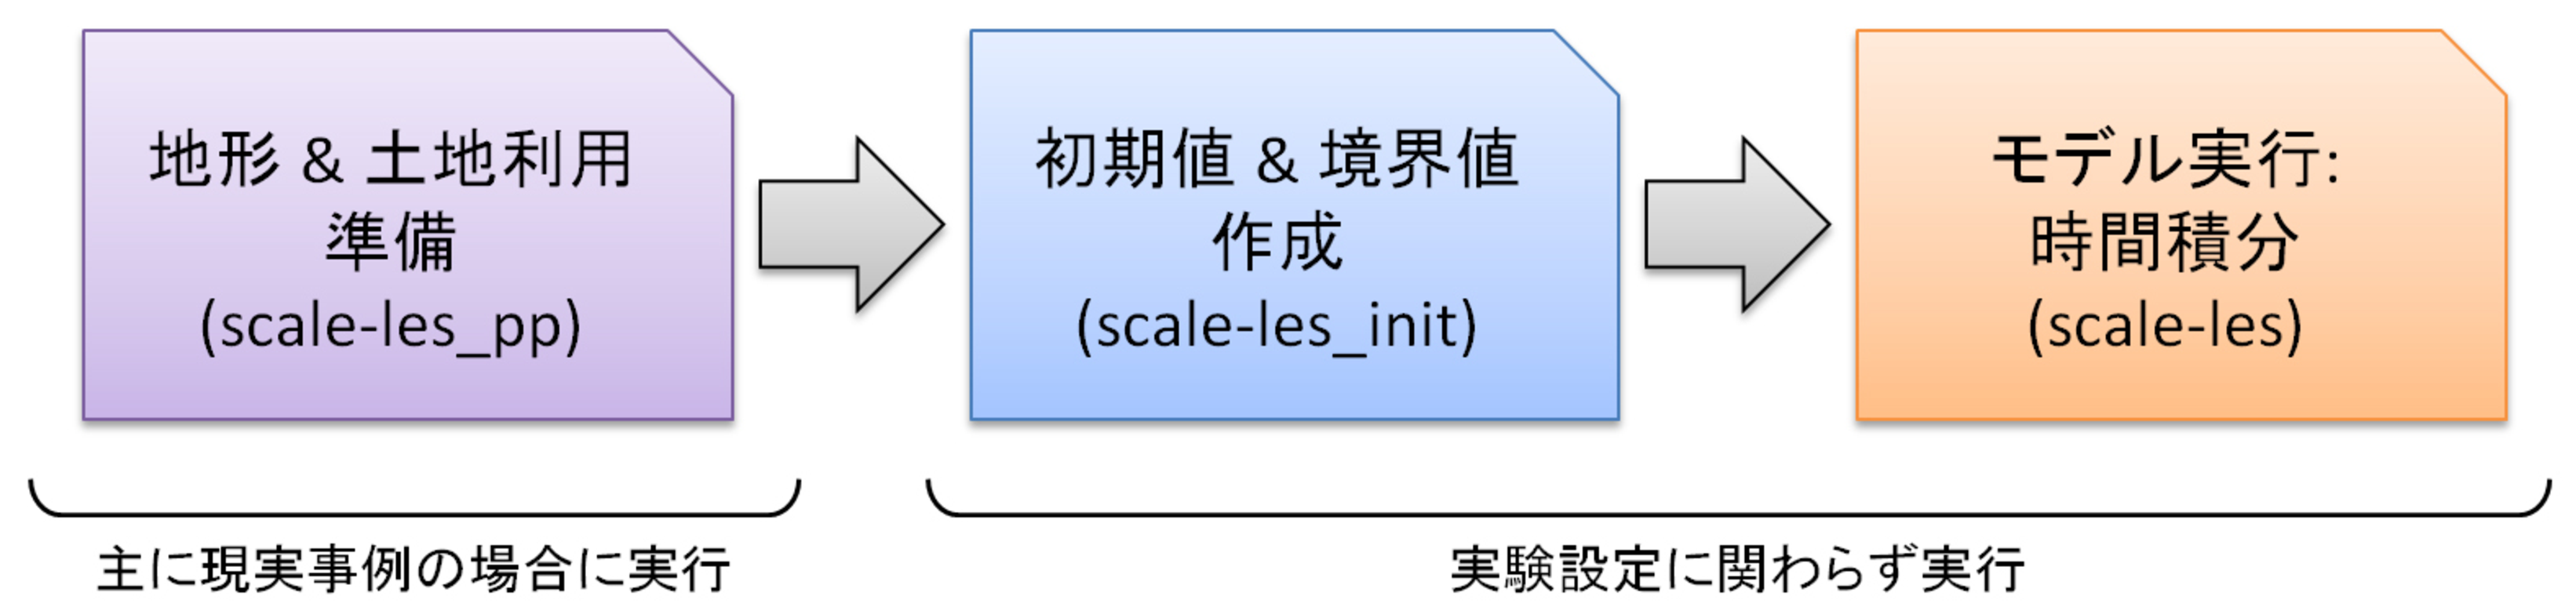
\includegraphics[width=0.9\hsize]{./figure/how_to_run.eps}\\
  \caption{SCALE-LESモデルの実行過程}
  \label{fig:howto}
\end{center}
\end{figure}



\section{理想実験の実行方法}
理想実験は
\begin{verbatim}
  scale/uguide/scale/scale-les/test/case/
\end{verbatim}
にいくつか用意されている。
\ref{sec:req_env}の実行環境で動かせる理想実験は、
今日時点ではないため、使い方のみ説明する。


\subsubsection{コンパイル}
実験したい実験のディレクトリに移動して、コンパイルする.
\begin{verbatim}
  $ cd scale/uguide/scale/scale-les/test/case/HOGEHOGE/
  $ make -j 4
\end{verbatim}

\subsubsection{実行方法}
理想実験は,コンパイルが完了したディレクトリ上で,下記のコマンドによって
実行することができる.
\begin{verbatim}
  $ make run
\end{verbatim}
この場合,デフォルトのconfigurationファイルを使用して自動的に実験設定に
合った初期値・境界値を作成し,その後scale-lesモデル本体を実行する.
"make run"のコマンドを使用せず,以下のように手動で実行過程を進めることもできる.

\begin{enumerate}
\item 実験設定を記述したconfigurationファイル,init.confを編集して目的の実験にあった設定を構築する.

\item 下記のコマンドによって事前処理(初期値・境界値作成)を実行する.ここの例ではMPI並列として6プロセスを使用している.
\begin{verbatim}
$ mpirun -n 6 ./scale-les_init init.conf
\end{verbatim}
正常にJOBが終了すれば,
\verb|init_****.pe#####.nc|,および\verb|boundary.pe#####.nc|
といったファイルが,それぞれMPIプロセス数ずつ生成される(\verb|#####|はMPIプロセスの番号).

\item モデルを実行するためにrun.confを適宜編集する.MPIプロセスの数や,格子,境界の取り方の設定については,init.confの時の設定と相違ないように注意すること.
正常にJOBが終了すれば,\verb|init_****.pe#####.nc|,
および\verb|boundary.pe#####.nc|といったファイルが,それぞれMPIプロセス数ずつ生成される(\verb|#####|はMPIプロセスの番号).

\item 下記のコマンドによってモデルを実行する.
\begin{verbatim}
$ mpirun -n 6 ./scale-les run.conf
\end{verbatim}
configurationファイルの設定によるが,\verb|history.pe#####.nc|
という名前のファイルが作成され,この中に出力変数が含まれている.
\end{enumerate}


\section{現実大気実験の実行方法}
%====================================================================================

このチュートリアルでは,Fig. \ref{fig:domain}に示した日本域を対象とした
現実大気実験を行う.
計算領域(ドメイン)の設定はTable \ref{tab:grids}のようになっている.

\begin{figure}[h]
\begin{center}
  \includegraphics[width=0.5\hsize]{./figure/domain.eps}\\
  \caption{計算領域.コンターは海岸線,カラーシェードは地形の高度を示す.}
  \label{fig:domain}
\end{center}
\end{figure}

\begin{table}[h]
\begin{center}
  \caption{実験設定の概略}
  \label{tab:grids}
  \begin{tabularx}{150mm}{|l|X|} \hline
    \rowcolor[gray]{0.9} 項目 & 設定 \\ \hline
    MPIプロセス分割 (東西 x 南北) & 3 x 3 (合計9プロセス) \\ \hline
    水平格子数 (東西 x 南北) & 180格子点 x 180格子点 \\ \hline
    鉛直層数                 & 36層                  \\ \hline
    水平格子間隔             & dx = dy = 7500m       \\ \hline
    積分期間 & 1999年5月5日 00UTC~12UTC (12時間積分) \\ \hline
    時間ステップ間隔 & 30 sec (1440 steps) \\ \hline
  \end{tabularx}
\end{center}
\end{table}



\subsection{地形・土地利用データの作成:pp}
%-----------------------------------------------------------------------------------

ここでは,\ref{sec:source_code}節でダウンロードした\verb|tutorial_data|は,
\verb|${TOPDIR}/data/|の下に展開されていると想定している.

まず,ppディレクトリへ移動する.
ppでは現実実験のための地形データ、土地利用データを作成する.
\begin{verbatim}
 $ cd scale/scale-les/test/tutorial/pp
\end{verbatim}
ppディレクトリの中には,\verb|pp.conf|という名前の
コンフィグファイルが準備されている.
地球上でのドメインの位置や格子点数など、実験設定に合わせて,
適宜\verb|pp.conf|を編集する必要があるが,
チュートリアルでは,すでに編集済みの\verb|pp.conf|が
与えられているためそのまま利用する.
\verb|pp.conf|の設定の中で特に注意するべき項目は,\verb|PARAM_CONVERT|である.
\begin{verbatim}
 &PARAM_CONVERT
  CONVERT_TOPO = .true.,
  CONVERT_LANDUSE = .true.,
 /
\end{verbatim}
上記のように\verb|CONVERT_TOPO|と\verb|CONVERT_LANDUSE|が
\verb|.true.|となっていることが,
それぞれ地形と土地利用の処理を行うことを意味している.
詳細なコンフィグファイルの内容については,
Appendix \ref{app:namelist}を参照されたい.

次に,コンパイル済みのバイナリと入力データをppディレクトリへリンクする.
\begin{verbatim}
 $ ln -s ${TOPDIR}/bin/scale-les_pp ./
 $ ln -s ${TOPDIR}/data/tutorial_data/data/input_topo    ./
 $ ln -s ${TOPDIR}/data/tutorial_data/data/input_landuse ./
\end{verbatim}
今回は,Table \ref{tab:grids}に示されているように,
9つのMPIプロセスを使用する設定なので次のように実行する.
\begin{verbatim}
 $ mpirun -n 9 ./scale-les_pp pp.conf
\end{verbatim}
正常にジョブが終了すれば,\verb|topo_d01.pe######.nc|と\verb|landuse_d01.pe######.nc|というファイルがMPIプロセス数だけ,つまり9つずつ生成される(\verb|######|にはMPIプロセスの番号が入る).
それぞれ,ドメインの格子点に内挿された地形と土地利用の情報が入ってる.

処理内容のログとして,\verb|pp_LOG_d01.pe000000|という名前でログファイルも
出力されるので内容を確かめておくこと.
gpviewがインストールされていれば,次のコマンドによって作成された地形と土地利用データを
描画してチェックすることができる.
正しく作成されていれば,Fig. \ref{fig:domain}と同じように描かれる.
\begin{verbatim}
$ gpview topo_d01.pe00000*@TOPO --aspect=1
$ gpview landuse_d01.pe00000*@FRAC_LAND --aspect=1
\end{verbatim}


\subsection{初期値・境界値データの作成:init}
%-----------------------------------------------------------------------------------

init では,SCALE計算に必要な初期値・境界値データを作成する.
まず,initディレクトリへ移動する.
\begin{verbatim}
 $ cd scale/scale-les/test/tutorial/init
\end{verbatim}

initディレクトリの中には,\verb|init.conf|という名前のコンフィグファイルが準備されている.
\verb|pp.conf|と同様に,実験設定に合わせて、この\verb|init.conf|を書き換える必要があるが、
チュートリアル用の\verb|init.conf|ファイルはTable\ref{tab:grids}の設定に
すでに合わせてある.
初期値・境界値データの作成には前節で作成した地形・土地利用データを利用する.
これは,下記のように,相対PATHを用いて参照するように設定されている.

\begin{verbatim}
&PARAM_TOPO
 TOPO_IN_BASENAME = "../pp/topo_d01",
/
&PARAM_LANDUSE
 LANDUSE_IN_BASENAME  = "../pp/landuse_d01",
/
\end{verbatim}
その他に\verb|init.conf|の設定の中で特に注意するべき項目は,
\verb|PARAM_MKINIT_REAL|である.

\begin{verbatim}
&PARAM_MKINIT_REAL
 BASENAME_BOUNDARY   = "boundary_d01",  <- 境界値データの出力名
 FILETYPE_ORG        = "NICAM-NETCDF",
 NUMBER_OF_FILES     = 2,               <- 読み込むファイルの数
 BOUNDARY_UPDATE_DT  = 21600.D0,        <- 入力データの時間間隔
 INTERP_SERC_DIV_NUM = 20,              <- 内挿計算用のチューニングパラメータ
/
\end{verbatim}

\verb|FILETYPE_ORG|は入力する気象場データのファイルフォーマットに
関するパラメータを設定しており,ここでは
NICAMモデルのnetcdf形式データのフォーマットで読み込むことを指定している.
詳細なコンフィグファイルの内容については,Appendix \ref{app:namelist}を参照されたい.

次に,コンパイル済みのバイナリをinitディレクトリへリンクする.
\begin{verbatim}
 $ ln -s ${TOPDIR}/bin/scale-les_init ./
\end{verbatim}
入力データはinitディレクトリの中に準備されている,\verb|"inputdata-link.sh"|を用いてリンクする.
\begin{verbatim}
 $ sh inputdata-link.sh
\end{verbatim}
としてスクリプトを実行することで,気象場の入力データがリンクされ,initディレクトリ内に下記のファイルがリンクされる.
このスクリプトにあるstart dateとend dateの設定項目を実験設定に対応するように編集するが、ここでは,start dateは1999/05/05 00:00:00,end dateは1999/05/06 00:00:00と設定している.もし,\verb|tutorial_data|を\verb|${TOPDIR}/data|以外の場所に展開している場合は,スクリプト内の
\verb|"dir"|の項目も適切なディレクトリに変更すること.下記ファイルにリンクが張れれば成功.
{\small
\begin{verbatim}

la_tg_00000.peall.nc    ms_qv_00000.peall.nc   oa_sst_00000.peall.nc  ss_tem_sfc_00000.peall.nc
la_tg_00001.peall.nc    ms_qv_00001.peall.nc   oa_sst_00001.peall.nc  ss_tem_sfc_00001.peall.nc
la_wg_00000.peall.nc    ms_tem_00000.peall.nc  ss_q2m_00000.peall.nc  ss_u10m_00000.peall.nc
la_wg_00001.peall.nc    ms_tem_00001.peall.nc  ss_q2m_00001.peall.nc  ss_u10m_00001.peall.nc
lsmask_00000.peall.nc   ms_u_00000.peall.nc    ss_slp_00000.peall.nc  ss_v10m_00000.peall.nc
lsmask_00001.peall.nc   ms_u_00001.peall.nc    ss_slp_00001.peall.nc  ss_v10m_00001.peall.nc
ms_pres_00000.peall.nc  ms_v_00000.peall.nc    ss_t2m_00000.peall.nc
ms_pres_00001.peall.nc  ms_v_00001.peall.nc    ss_t2m_00001.peall.nc

\end{verbatim} }

次に、陸面過程や放射過程のモデルを起動するためのパラメータファイルにリンクをはる.
\begin{verbatim}
 $ ln -s scale/scale-les/test/data/land/*  ./
 $ ln -s scale/scale-les/test/data/rad/*   ./
\end{verbatim}
上の行のリンクコマンドによって陸面過程のパラメータファイルがリンクされ,
下の行のコマンドによって放射過程のパラメータファイルがリンクされる.
準備が整ったら,9つのMPIプロセスを使用してinitを実行する.
\begin{verbatim}
 $ mpirun -n 9 ./scale-les_init init.conf
\end{verbatim}

正常にジョブが終了すれば,
\verb|boundary_d01.pe######.nc|と\verb|init_d01_00010713600.000.pe######.nc|というファイルが
MPIプロセス数だけ,つまり9つずつ生成される(\verb|######|にはMPIプロセスの番号が入る).
それぞれ,境界値データと初期値データが入ってるおり,境界値データには複数の時刻のデータが1つのファイルに含まれている.
初期値ファイルの名前のうち\verb|"00010713600.000"|の部分は,モデル内で算出された実験開始時刻を表している.

処理内容のログとして,\verb|init_LOG_d01.pe000000|という名前でログファイルも出力されるので内容を確かめておくこと.
gpviewがインストールされていれば,次のコマンドによって作成された地形と土地利用データを描画してチェックすることができる.
正しく作成されていれば,Fig. \ref{fig:init}と同じように描かれる.

\begin{verbatim}
$ gpvect --scalar --slice z=1500 --nocont --aspect=1 --range=0.001:0.015          \
         --xintv=10 --yintv=10 --unit_vect init_d01_00010713600.000.pe00*@QV      \
         init_d01_00010713600.000.pe00*@MOMX init_d01_00010713600.000.pe00*@MOMY
\end{verbatim}


\begin{figure}[h]
\begin{center}
  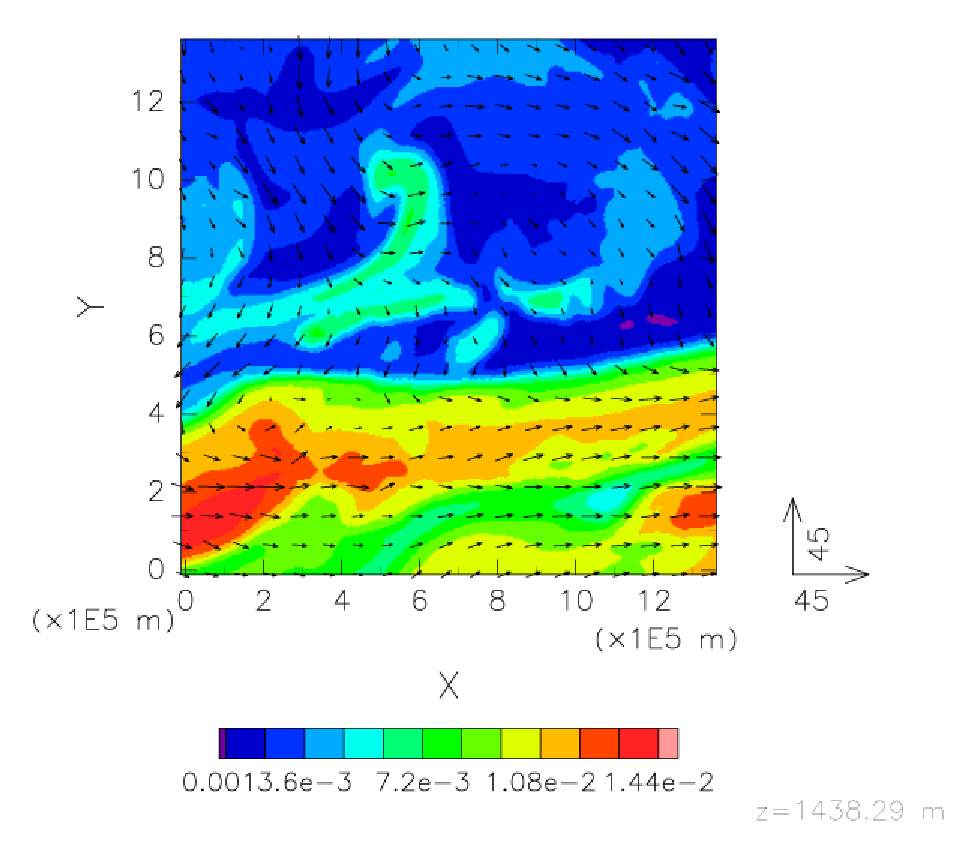
\includegraphics[width=0.7\hsize]{./figure/init_qv-momxy.eps}\\
  \caption{チュートリアル実験の初期場の様子:カラーシェードは高度1.5kmにおける比湿の分布,ベクトルは高度1.5kmにおける水平運動量フラックスを表している.}
  \label{fig:init}
\end{center}
\end{figure}


\subsection{時間積分を行う:run}
%-----------------------------------------------------------------------------------

ここではいよいよSCALE-LESモデルを実行する.
まず,runディレクトリへ移動する.
\begin{verbatim}
  $ cd scale/scale-les/test/tutorial/run
\end{verbatim}


runディレクトリの中には,これまでと同様に\verb|run.conf|という名前のコンフィグファイルが準備されている.
チュートリアル用の\verb|run.conf|ファイルのドメインの位置や格子点数などはTable\ref{tab:grids}の設定に合わせてある.
モデル本体の実行には事前に作成した地形・土地利用データや初期値・境界値データを利用する.
これらのファイルを参照するために,
\verb|TOPO_IN_BASENAME|,\verb|LANDUSE_IN_BASENAME|,
\verb|RESTART_IN_BASENAME|,および\verb|ATMOS_BOUNDARY_IN_BASENAME|で
それぞれ場所を指定する.

\begin{verbatim}
&PARAM_TOPO
 TOPO_IN_BASENAME = "../pp/topo_d01",
/

&PARAM_LANDUSE
 LANDUSE_IN_BASENAME  = "../pp/landuse_d01",
/

&PARAM_RESTART
 RESTART_OUTPUT      = .false.,
 RESTART_IN_BASENAME = "../init/init_d01_00010713600.000",
/

&PARAM_ATMOS_BOUNDARY
 ATMOS_BOUNDARY_TYPE        = "REAL",
 ATMOS_BOUNDARY_IN_BASENAME = "../init/boundary_d01",
 ATMOS_BOUNDARY_USE_VELZ    = .true.,
 ATMOS_BOUNDARY_USE_QHYD    = .false.,
 ATMOS_BOUNDARY_VALUE_VELZ  = 0.0D0,
 ATMOS_BOUNDARY_UPDATE_DT   = 21600.0D0,
/

\end{verbatim}


\verb|run.conf|の設定の中で時間積分に関する設定は,\verb|PARAM_TIME|の項目にある.
\begin{verbatim}
&PARAM_TIME
 TIME_STARTDATE             = 1999, 5, 5, 0, 0, 0,
 TIME_STARTMS               = 0.D0,
 TIME_DURATION              = 12.0D0,
 TIME_DURATION_UNIT         = "HOUR",
 TIME_DT                    = 30.0D0,
 TIME_DT_UNIT               = "SEC",
 TIME_DT_ATMOS_DYN          = 7.5D0,
 TIME_DT_ATMOS_DYN_UNIT     = "SEC",

 ~~中略~~

/
\end{verbatim}

\verb|TIME_STARTDATE|は時間積分を開始する時刻を設定する項目で,チュートリアルでは1999年5月5日0時UTCと設定する.
\verb|TIME_DURATION|は積分期間を設定する項目で,ここでは12時間積分を行う設定になっている.
\verb|TIME_DT|,および\verb|TIME_DT_ATMOS_DYN|は,時間積分の間隔(時間ステップ間隔:DT = Delta Time)を設定する項目である.前者は移流計算,後者はそれ以外の力学過程の計算に関する時間積分間隔である.
SCALE-LESモデルでは,そのほかの物理過程についても細かく時間積分間隔を設定できるようになっている.


出力データに関する設定は\verb|PARAM_HISTORY|で行う.

\begin{verbatim}
&PARAM_HISTORY
 HISTORY_DEFAULT_BASENAME  = "history_d01",
 HISTORY_DEFAULT_TINTERVAL = 1800.D0,
 HISTORY_DEFAULT_TUNIT     = "SEC",
 HISTORY_DEFAULT_TAVERAGE  = .false.,
 HISTORY_DEFAULT_DATATYPE  = "REAL4",
 HISTORY_DEFAULT_ZINTERP   = .true.,
/
\end{verbatim}

\verb|HISTORY_DEFAULT_BASENAME|は出力するファイル名である.
\verb|HISTORY_DEFAULT_TINTERVAL|と\verb|HISTORY_DEFAULT_TUNIT|によってヒストリー出力時間間隔が設定される.
ここでは1800秒(30分)間隔での出力として設定されている.
この設定で,\verb|HISTITEM|として羅列された変数について出力される.
\verb|HISTITEM|では、オプション変数を加えることで、出力間隔を変数毎に変更したり、平均値を出力したりすることも出来る。
これらの説明は\ref{sec:output}を参照されたい.

\begin{verbatim}
&HISTITEM item="DENS" /           ! density (3D)
&HISTITEM item="MOMZ" /           ! vertical momentum (3D)
&HISTITEM item="MOMX" /           ! horizontal momentum-x (3D)
&HISTITEM item="MOMY" /           ! horizontal momentum-y (3D)
&HISTITEM item="RHOT" /           ! density * potential-temperature (3D)

&HISTITEM item="QV"   /           ! mixing ratio for vapor (3D)
&HISTITEM item="QHYD" /           ! mixing ratio for hydrometeor (3D)

&HISTITEM item="T"    /           ! temperature (3D)
&HISTITEM item="PRES" /           ! pressure (3D)
&HISTITEM item="U"    /           ! horizontal wind component-x (3D)
&HISTITEM item="V"    /           ! horizontal wind component-y (3D)
&HISTITEM item="W"    /           ! vertical wind component (3D)
&HISTITEM item="PT"   /           ! potential temperature (3D)
&HISTITEM item="RH"   /           ! relative humidity (3D)

&HISTITEM item="PREC" /           ! precipitation (2D)
&HISTITEM item="OLR"  /           ! out-going longwave radiation

&HISTITEM item="U10" /            ! horizontal wind component-x at 10m height(2D)
&HISTITEM item="V10" /            ! horizontal wind component-y at 10m height(2D)
&HISTITEM item="T2"  /            ! temperature at 2m height (2D)
&HISTITEM item="Q2"  /            ! mixing ratio for vapor at 2m height (2D)

&HISTITEM item="SFC_PRES"   /     ! pressure at the bottom surface (2D)
&HISTITEM item="SFC_TEMP"   /     ! temperature a the bottom surface (2D)
&HISTITEM item="LAND_SFC_TEMP" /  ! temperature a the bottom surface for land model (2D)
&HISTITEM item="URBAN_SFC_TEMP" / ! temperature a the bottom surface for urban model (2D)

\end{verbatim}


その他に実験で使用される物理過程の設定は,
\verb|PARAM_TRACER,PARAM_ATMOS,PARAM_OCEAN,PARAM_LAND,PARAM_URBAN|の項目に
記述されているので,実行前にチェックすること.
詳細なコンフィグファイルの内容については,Appendix \ref{app:namelist}を参照されたい.


次に,コンパイル済みのバイナリをrunディレクトリへリンクする.

\begin{verbatim}
  $ ln -s ${TOPDIR}/bin/scale-les ./
\end{verbatim}

また,前節と同様に陸面過程や放射過程のモデルを起動するためのパラメータファイルも
リンクしておく.

\begin{verbatim}
  $ ln -s scale/scale-les/test/data/land/*  ./
  $ ln -s scale/scale-les/test/data/rad/*   ./
\end{verbatim}
上の行のリンクコマンドによって陸面過程のパラメータファイルがリンクされ,
下の行のコマンドによって放射過程のパラメータファイルがリンクされる.
準備が整ったら,9つのMPIプロセスを使用してscale-lesを実行する.
\begin{verbatim}
  $ mpirun -n 9 ./scale-les run.conf < /dev/null >&log&
\end{verbatim}


実行にはおおよそ2時間を要するため,上記のように標準出力をファイルへ
吐き出すようにしてバックグラウンドで実行しておくと便利である.
計算が開始されれば,処理内容のログとして,\verb|"LOG_d01.pe000000"|ファイルが生成されるので,
例えば下記のようなコマンドで\verb|"LOG_d01.pe000000"|ファイルを参照すれば,
どこまで計算が進んでいるかチェックすることができる.
\begin{verbatim}
  $ tail -n 50 LOG_d01.pe000000
\end{verbatim}
正常にジョブが終了すれば,\verb|history_d01.pe######.nc|と\verb|restart_d01.pe######.nc|と
いう名前のファイルがMPIプロセス数だけ,つまり9つずつ生成される
(\verb|######|にはMPIプロセスの番号が入る).
historyファイルは実行結果のプロダクトであり,restartファイルは対応する時刻を開始時刻として
再計算を開始するための初期値ファイルである.

次節でhistoryデータを描画して結果を調べる方法を説明する.

%####################################################################################


\section{Quicklook SCALE-LES output}
%####################################################################################

SCALE-LESモデルの出力ファイルはMPIプロセス毎に出力され,計算領域が分割された状態で出力されている.
ファイル自体のフォーマットは気候・予報(CF)メタデータ規約に対応したnetcdf4形式でアウトプットされている.
ここでは,gpviewとgradsを使用した2通りの描画方法について説明する。

\subsection{RubyDCL/Gphys: gplist, gpprint, gpview, gpvect}
%====================================================================================

Dennou系のRubyベースコマンドgpviewによって直接描画することができる.
RubyDCL/Gphysがインストールされていない場合は,Appendix \ref{sec:env_setting}を参照して
事前にインストールすること.
以下にチュートリアルで実行した結果を描画する方法についていくつか例を挙げる.


\subsubsection{ファイル内の変数を確認する}
%-----------------------------------------------------------------------------------

まず,gplistコマンドを用いてヒストリーファイル内の変数を確認する.

\begin{verbatim}
$ gplist history_d01.pe000000.nc
\end{verbatim}

\verb|history_d01.pe######.nc|のファイルはMPI並列数分だけ存在するが,
ファイルに収められている変数は基本的に同じであるため,
どれか1つのファイルについて中身を確認すればよい.
上記のコマンドを実行すると,下記のように変数リストが表示される.

{\small \begin{verbatim}
history_d01.pe000000.nc:
  x	[x=62]	'X'	(m)
  y	[y=62]	'Y'	(m)
  z	[z=36]	'Z'	(m)
  xh	[xh=62]	'X (half level)'	(m)
  yh	[yh=62]	'Y (half level)'	(m)
  zh	[zh=36]	'Z (half level)'	(m)

 ~~中略~~

  topo	[x=62,y=62]	'topography'	(m)
  lsmask	[x=62,y=62]	'fraction for land-sea mask'	(0-1)
  time	[time=24]	'time'	(seconds since 1999-01-01 00:00:00)
  time_bnds	[nv=2,time=24]	''	(seconds since 1999-01-01 00:00:00)
  DENS	[x=62,y=62,z=36,time=24]	'density'	(kg/m3)
  MOMZ	[x=62,y=62,zh=36,time=24]	'momentum z'	(kg/m2/s)
  MOMX	[xh=62,y=62,z=36,time=24]	'momentum x'	(kg/m2/s)
  MOMY	[x=62,yh=62,z=36,time=24]	'momentum y'	(kg/m2/s)
  RHOT	[x=62,y=62,z=36,time=24]	'rho * theta'	(kg/m3*K)
  QV	[x=62,y=62,z=36,time=24]	'Water Vapor mixing ratio'	(kg/kg)
  W	[x=62,y=62,z=36,time=24]	'velocity w'	(m/s)
  U	[x=62,y=62,z=36,time=24]	'velocity u'	(m/s)
  V	[x=62,y=62,z=36,time=24]	'velocity v'	(m/s)
  PT	[x=62,y=62,z=36,time=24]	'potential temp.'	(K)
  QHYD	[x=62,y=62,z=36,time=24]	'total hydrometeors'	(kg/kg)
  PRES	[x=62,y=62,z=36,time=24]	'pressure'	(Pa)
  T	[x=62,y=62,z=36,time=24]	'temperature'	(K)
  RH	[x=62,y=62,z=36,time=24]	'relative humidity'	(%)
  PREC	[x=62,y=62,time=24]	'surface precipitation rate'	(kg/m2/s)
  OLR	[x=62,y=62,time=24]	'TOA net longwave  radiation flux'	(W/m2)

 ~~中略~~
\end{verbatim} }

x, y, zなどの変数は格子情報を表しており,\verb|DENS, MOMZ, MOMX|や
\verb|PT, QHYD, PRES|といった変数が気象場のデータである.
この中から1つ,もしくは複数の変数を選んで描画する.

各気象場の変数に対してデータの軸構成が書かれている.
例えば,\verb|DENS|は空間を構成するx軸,y軸,z軸と時間を構成するtime軸によってデータが構成されている.
高度や時刻を指定して描画するためには,このようにデータを構成する軸についてあらかじめ知っておく必要がある.
例えばヒストリー出力されている時刻を調べるには次のようにコマンドを実行する.

\begin{verbatim}
$ gpprint history_d01.pe000000.nc@time
\end{verbatim}

そうすると下記のようにtime変数の値が標準出力へ表示される.

\begin{verbatim}
 1.07154e+07, 1.07172e+07, 1.0719e+07, 1.07208e+07, 1.07226e+07, 1.07244e+07,
 1.07262e+07, 1.0728e+07, 1.07298e+07, 1.07316e+07, 1.07334e+07, 1.07352e+07,
 1.0737e+07, 1.07388e+07, 1.07406e+07, 1.07424e+07, 1.07442e+07, 1.0746e+07,
 1.07478e+07, 1.07496e+07, 1.07514e+07, 1.07532e+07, 1.0755e+07, 1.07568e+07,
\end{verbatim}

SCALE-LESモデル内では日時が全て秒単位で表現されているため,ここで表記される
時刻も日時が全て秒として積算された値が時刻として表示される.
SCALE-LESモデルはデフォルト設定で,一番始めに初期値がヒストリー出力され,
そのあと\verb|HISTORY_DEFAULT_TINTERVAL|に従った時間間隔でヒストリー出力されている.
チュートリアルでは12時間積分する中で,30分ごとに出力したため,
1(初期値)+23ステップ=24ステップの時刻のデータが出力されていることがわかる.


{\small *netcdfに付属している\verb|"ncdump"|を用いてもよい.}


\subsubsection{ファイル内の変数を描画する}
%-----------------------------------------------------------------------------------

gpviewを用いて次のように描画できる.

(例 1)高度1500mにおける温度の水平分布
\begin{itemize}

\item 積分開始3時間後の様子
  \begin{verbatim}
  gpview history_d01.pe00000*@T,z=1500,time=1.07262e+07 --range=270:291 --aspect=1
  \end{verbatim}
  実行結果はFig. \ref{fig:hist_t}aのようになる(画面をクリックするか\verb|"q"|を打つことで終了する).
  オプションの\verb|z=1500,time=1.07262e+07|によって描画する高度,および時刻を指定している.
  \verb|--range=270:291|のオプションは描画する値のレンジを指定している.
  また,\verb|"--wsn=2"|のオプションを付けて実行することで,\verb|"dcl.ps"|というファイル名で
  画像をPSファイルに保存することができる.

\item 積分開始6時間後の様子:実行結果はFig. \ref{fig:hist_t}bのようになる.
  \begin{verbatim}
  gpview history_d01.pe00000*@T,z=1500,time=1.0737e+07 --range=270:291 --aspect=1
  \end{verbatim}
  先との変更点はtimeオプションの引数だけである.

\item 積分開始9時間後の様子:実行結果はFig. \ref{fig:hist_t}cのようになる.
  \begin{verbatim}
  gpview history_d01.pe00000*@T,z=1500,time=1.07478e+07 --range=270:291 --aspect=1
  \end{verbatim}

\end{itemize}


\begin{figure}[t]
\begin{center}
  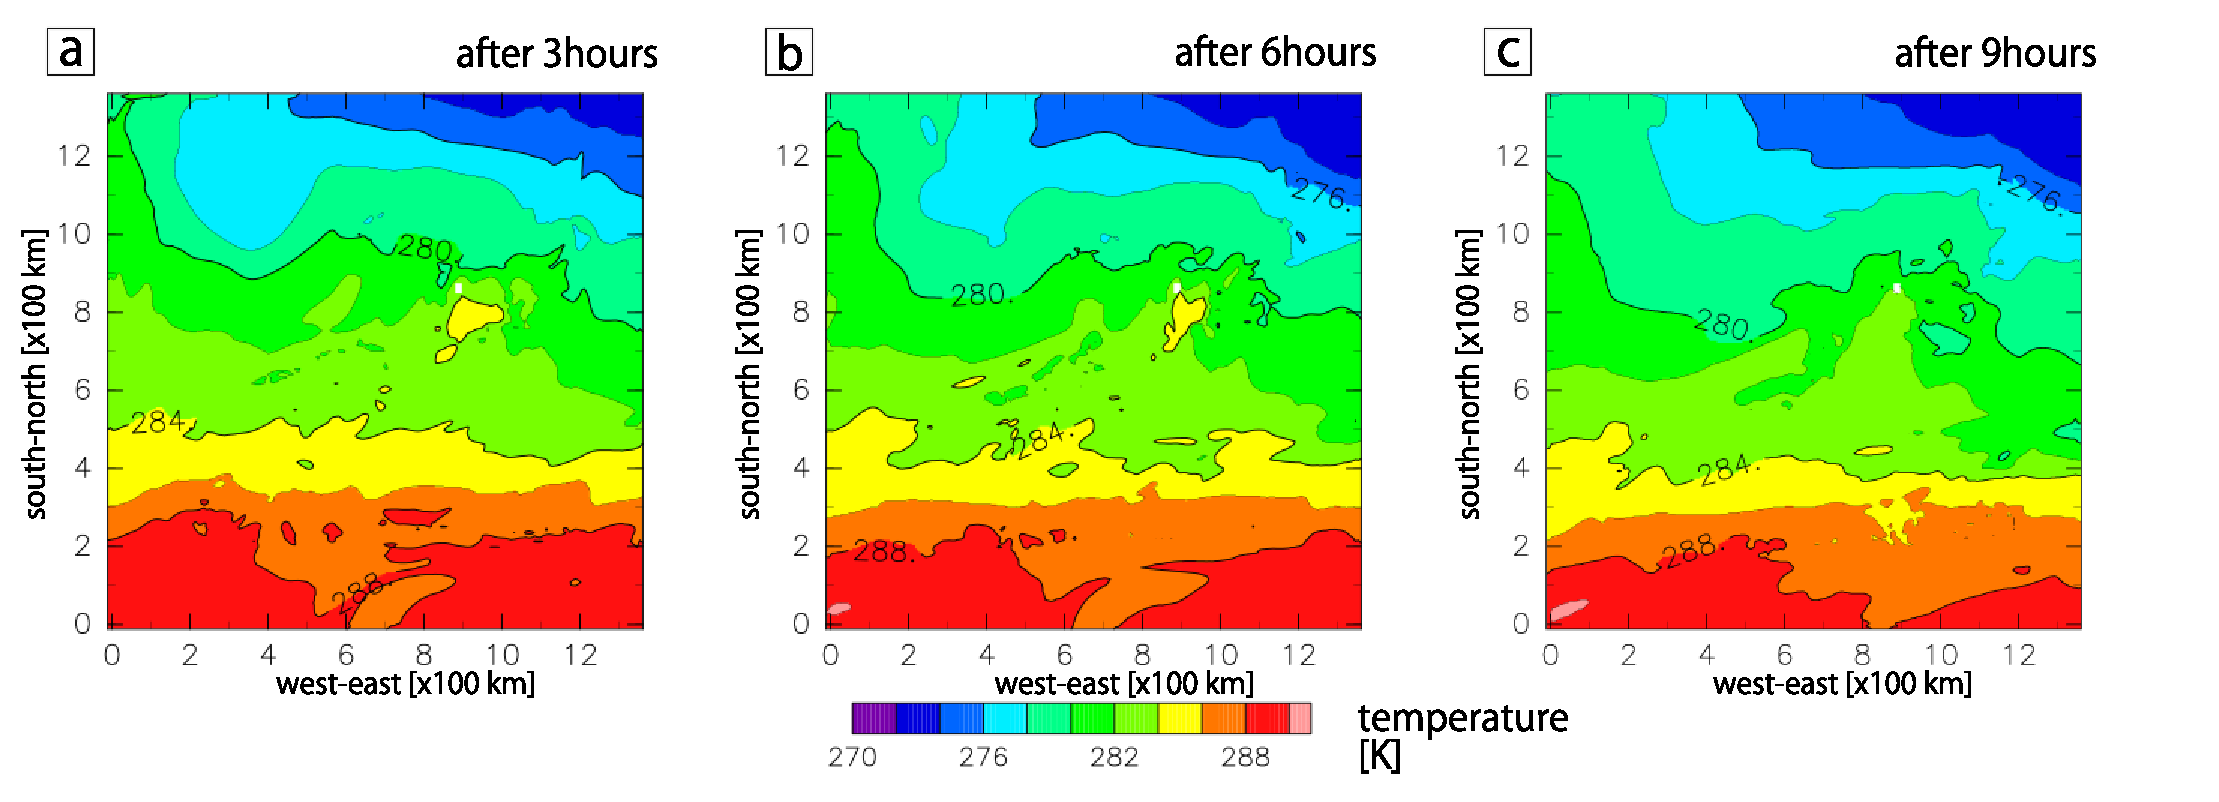
\includegraphics[width=0.9\hsize]{./figure/gpview_hist_t.eps}\\
  \caption{高度1.5kmにおける気温の分布}
  \label{fig:hist_t}
\end{center}
\end{figure}


(例 2)高度1500mにおける相対湿度と水平風の分布
\begin{itemize}

\item 積分開始3時間後の様子
  \begin{verbatim}
  gpvect --scalar --slice z=1500,time=1.07262e+07 --nocont --range=10:102        \
         --aspect=1 --xintv=10 --yintv=10 --unit_vect history_d01.pe00000*@RH    \
         history_d01.pe00000*@U history_d01.pe00000*@V
  \end{verbatim}
  実行結果はFig. \ref{fig:hist_rh}aのようになる.
  ここでは\verb|gpview|ではなくベクトルを描画することができる\verb|gpvect|を使用して描画する.
  オプションの\verb|--xintv=10 --yintv=10|は,ベクトルを描画する格子点間隔を指定している.

\item 積分開始6時間後の様子:実行結果はFig. \ref{fig:hist_rh}bのようになる.
  \begin{verbatim}
  gpvect --scalar --slice z=1500,time=1.0737e+07 --nocont --range=10:102        \
         --aspect=1 --xintv=10 --yintv=10 --unit_vect history_d01.pe00000*@RH    \
         history_d01.pe00000*@U history_d01.pe00000*@V
  \end{verbatim}

\item 積分開始9時間後の様子:実行結果はFig. \ref{fig:hist_rh}cのようになる.
  \begin{verbatim}
  gpvect --scalar --slice z=1500,time=1.07478e+07 --nocont --range=10:102        \
         --aspect=1 --xintv=10 --yintv=10 --unit_vect history_d01.pe00000*@RH    \
         history_d01.pe00000*@U history_d01.pe00000*@V
  \end{verbatim}
\end{itemize}


\begin{figure}[t]
\begin{center}
  \includegraphics[width=0.9\hsize]{./figure/gpview_hist_rh.eps}\\
  \caption{高度1.5kmにおける相対湿度と水平風の分布:カラーシェードは相対湿度,ベクトルは水平風を示す}
  \label{fig:hist_rh}
\end{center}
\end{figure}


(例 3)QHYD(凝結物の混合比)についての計算領域西端から800kmの地点における鉛直-南北断面図

\begin{verbatim}
gpview history_d01.pe00000*@QHYD,x=800000,y=100000:600000,z=0:16000,time=1.0737e+07
\end{verbatim}
積分開始6時間後の様子で,実行結果はFig. \ref{fig:hist_qhyd}のようになる.
オプションの\verb|x=800000,y=100000:600000,z=0:16000|によって,xは800kmの地点,
yは100kmから600kmの範囲,zは0kmから16kmの範囲を描画するように指定している.


その他の描画例を下記に挙げる.
\begin{itemize}

\item 水平風南北成分を描画する:\\
  高度1000m指定,カンバスの縦横比=1,コンターなし,変数の描画範囲=4.8~5.2 [m/s],
  時間軸をアニメーション(クリックで進む)\\
  \verb|$ gpview history.pe00*@V,z=1000 --aspect 1 --nocont --range=4.8:5.2 --anim time|

\item 水蒸気混合比の南北-鉛直断面図を描画する:\\
  東西方向に50kmの位置を指定,コンターなし,時間軸をアニメーション,\verb|"--Gaw"|のオプションに
 より自動でアニメが進む,横軸と縦軸を交換 (exch)\\
  \verb|$ gpview history.pe00*@QV,x=50000 --aspect 1 --nocont --anim time --Gaw --exch|

\end{itemize}


\begin{figure}[t]
\begin{center}
  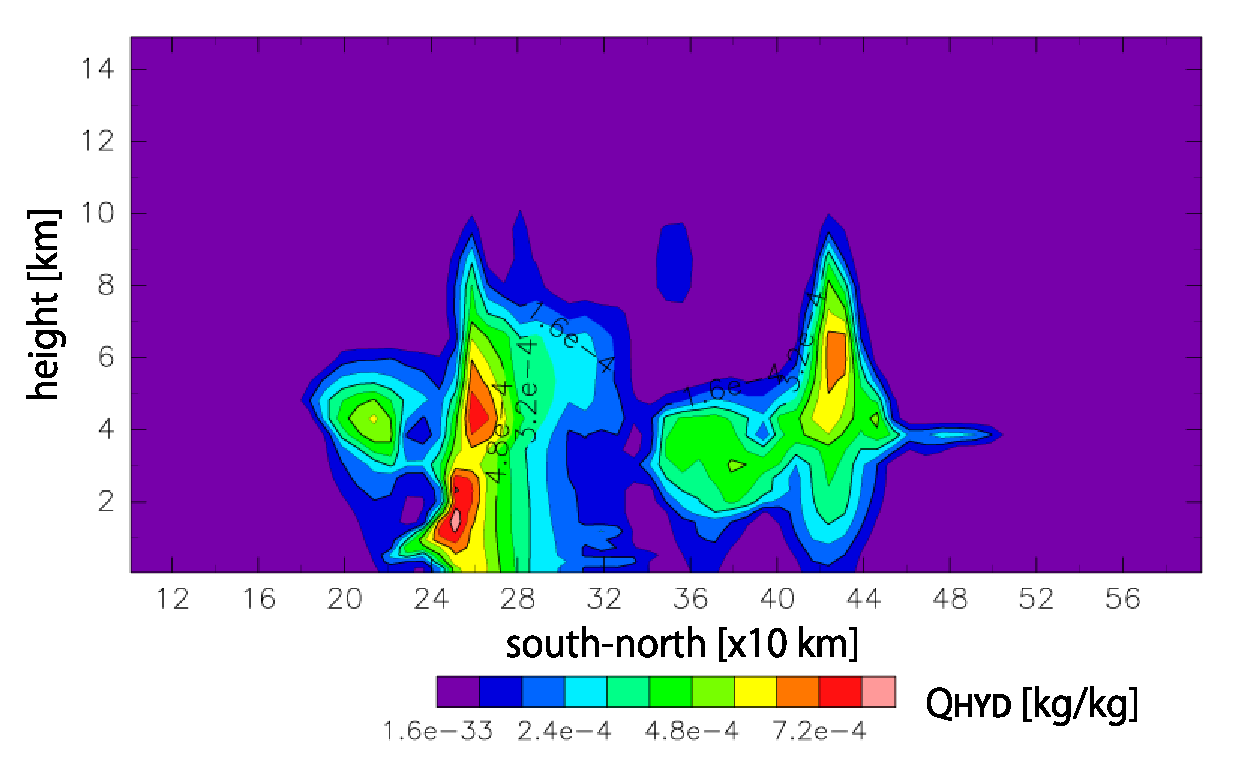
\includegraphics[width=0.7\hsize]{./figure/gpview_hist_qhyd.eps}\\
  \caption{x=800kmにおける鉛直-南北断面図}
  \label{fig:hist_qhyd}
\end{center}
\end{figure}


また,チュートリアルの中でも使用してきたが,下記のように\verb|init_****.pe#####.nc|ファイルなどを
指定することで,初期値・境界値や下端境界条件のファイルの中身も見ることが出来る.

\begin{itemize}
 \item \verb|$ gpview init_00000000000.000.pe00*@MOMX,z=1000 --aspect 1 --nocont|
 \item \verb|$ gpview boundary.pe00*@VELX,z=1000 --nocont --anim time|
 \item \verb|$ gpview topo.pe00*@TOPO --aspect 1|
 \item \verb|$ gpview landuse.pe00*@FRAC_LAND --aspect 1|
\end{itemize}


その他のオプション等については--helpを使ってヘルプを表示させるか,電脳倶楽部のWebページ
(\url{http://ruby.gfd-dennou.org/products/gphys/doc/gpview.html})を参照すること.


\subsection{netcdf2grads}
%====================================================================================

SCALE-LESの出力ファイル(\verb|history.******.nc|)を
GrADSで図化するためのnetcdf2grads の使用方法について説明する。
並列処理に対応したnetcdf2grads\_hも用意されているが、
ここではシングルノード用のnetcdf2gradsの使用方法を示す。
netcdf2grads\_h については、最後に簡単に説明する。
netcdf2gradsのソースファイルは \verb|scale/scale-les/util/netcdf2grads/|にある。
SCALE本体とは独立なので、ディレクトリを任意の場所に移動して
使用することが可能である.

\subsubsection{コンパイル}
\begin{description}
\item[Intel compiler]\mbox{}\\
 \begin{verbatim}
  ifort -convert big_endian -assume byterecl -I${NETCDF4}/include 
    -L${NETCDF4}/lib -lnetcdff -lnetcdf make_grads_file.f90 -o convine
  \end{verbatim}
\item[gfortran]\mbox{}\\
\begin{verbatim}
  gfortran -frecord-marker=4 --convert=big-endian -I${NETCDF4}/include
    -L${NETCDF4}/lib -lnetcdff -lnetcdf make_grads_file1.f90 -o convine
\end{verbatim}
\end{description}


\subsubsection{使用方法}
実行時に,インタラクティブモードかサイレントモードかを選択することが出来る.
\begin{verbatim}
   Interactive mode :  ''./convine -i''
   Silent mode      :  ''./convine -s''
\end{verbatim}
\begin{description}
\item[インタラクティブモード]\mbox{}\\
\begin{verbatim}
  cd netcdf2grads/
  ./convine -i
\end{verbatim}
と実行すると、下記のメッセージが出るので、指示通り、必要なファイルのパスを打ち込む.
\begin{verbatim}
path to configure file for run with the quotation mark
 '${path to directory of configure file}/run.conf' <- configureファイルへのパス
path to directory of history files with the quotation mark
 '${path to directory of history files}/' <- SCALE-LESの出力ファイルのパス
path to directory of output files with the quotation mark
 './grads/'  <- gradsファイルの出力先
start time of convert data
 1           <- 任意の番号の時間から変換可能. 
end time of convert data
 10          <- 変換を修了する時間
Imput number of variable
0 -> all variable output from model
 X           <- 変換したい変数の数
Imput variable
 VARIABLE(PRECなど)  <- 変換したい変数名
\end{verbatim}
うまく実行されれば、指定した出力先にctlファイルとgrdファイルが作成される。
\item[サイレントモード]\mbox{}\\
サイレントモードの場合は、あらかじめ、\verb|namelist.in|に必要な情報を書き入れておく.
\begin{verbatim}
  cd netcdf2grads/
  ./convine -s
\end{verbatim}
と実行すれば変換が始まる。
\end{description}



\subsubsection{並列処理: netcdf2grads\_h}

スパコンなどの大型計算機で並列計算を行った場合、
出力ファイルの数が多く、それぞれのファイルのデータ容量も大きい。
netcdf2gradsを並列処理したい場合にはこちらを使用する。
ここでは、K上での使用方法を簡単に説明する。

\begin{enumerate}
\item ファイルをコピー\\
 \verb|scale/scale-les/util/netcdf2grads_h| を \verb|/data/GROUP/USER/WORK_directory/| など、作業したいディレクトリにコピー。
\item コンパイル\\
 \verb|.bashrc| などに下記を設定
 \begin{verbatim}
  #--SCALE
   export SCALE_SYS=''K''
   export AGGRESIVE=''F''
   export FAST=''T''
   export DEBUG=''F''
 \end{verbatim}
 そして、コンパイル.\\
 \verb|$ make|\\
 うまくいけば、\verb|net2g|が作成される。
\item \verb|microで実行する| \\
 \verb|/scratch/GROUP/USER/|の下に、作業ディレクトリを用意する。そこに、
 \begin{verbatim}
   net2g         : copy executive file
   net2g.conf    : copy configure file
   output/  : link to directory with scale history files
   bindata/      : create directory for grads file output
   job.sh        : job script for K (option)
 \end{verbatim}
 を用意する。\verb|net2g.conf|の設定と\verb|job.sh|の設定をする。
 使用するノード数は、計算に使用したノード数の約数である必要がある。
\end{enumerate}


%####################################################################################




\chapter{SCALE-LES Advance use}
\section{任意のデータをSCALEで使用する}

\subsection{Topography and Landuse}

現在のSCALEでは用意されている地形・土地利用データよりも
高い解像度での計算ができない。

高解像度計算のためには、ユーザーが適宜データを用意する必要がある。


scale-lesでは日本領域については国土地理院のデータをもとにした地形,土地利用に関するデータベースを別途提供している(2.2節を参照).





\subsection{Initial and Boundary data}
\label{sec:adv_bnddata}

現在,scale-lesではWRF-ARWモデル,NICAM,およびscale-lesのデータを外部データとして初期値・境界値を作成する事ができる.
grads format dataの作成方法について説明

\section{実験設定の変更方法}
\subsection{Domain setting}

\subsection{Online nesting}

Online Nestingを行う場合は,Nestingの段数分だけpp.conf,init.conf,run.confファイルをそれぞれ用意する必要がある.
それぞれのドメイン毎に地形,土地利用,初期値・境界値を作成し,一番外側のドメインを下記のコマンドによって起動すると,
外側のドメインが順次,内側のドメインを起動する.
configureファイルの記述例はscale-les/test/case\_real/kobe\_prodの下にあるので適宜参照して欲しい.
\begin{verbatim}
$ mpirun -n 6 ./scale-les run.d01.conf
\end{verbatim}
このとき注意することは,Online Nesting計算の場合,実際に起動されるMPIプロセス数は外側のドメインを起動する時に指定したプロセス数(np)とドメイン段数を掛けた数になる.
たとえば,上記のコマンドで3段ドメインのOnline Nesting計算を行うことを考えると,total\_mpi\_processes = 3 (domain levels)×6 (np) = 36 processesとなる.
実行時のマシン環境に合わせて実験を行う必要がある.


\section{Description of namelist variables}
\subsection{Dynamical and Physical schemes}

ここでは、主要な数値スキームを変更する場合の仕方と種類について説明する。

\subsection{Setting of output variables to history file}
出力ファイルへの変数の追加は、2段階の手続きが必要である。
\begin{enumerate}
\item ソースファイル内の設定。対象の変数をhistory出力するための設定で、この手続きにより、出力のための準備が行われる。
\item run.conf内の設定。実際にhistoryに出力するかどうかを指定。コンパイルし直すことなく、実験毎に変更可能。
\end{enumerate}
予報変数や主要な変数についてはすでに1の手続きは行われているため、2だけを行えばよい。
対象となる変数リストは、Appendix\ref{app:vari_hist}を参照。
これ以外の変数をユーザーが書き出したい場合は、1の手続きが必要であるが、ここでは2の手続きのみ説明する。


出力ファイルへの変数の追加は、下記のフォーマットに従ってrun.confに追記すればよい。
%\begin{screen}
\begin{verbatim}
 &HISTITEM ITEM     = "character"
         (,BASENAME = "character",
           TINTERVAL= real,
           TUNIT    = "character", 
           TAVERAGE = logical,
           ZINTERP  = logical, 
           DATATYPE = "character")
 /
\end{verbatim}
%\end{screen}
$\left( \right)$内はオプション。
特に指定がない場合には、\verb|&PARAM_HISTORY|の設定がdefaultとして設定される。
%\begin{screen}
\begin{verbatim}
 &PARAM_HISTORY
  HISTORY_DEFAULT_BASENAME  = "character",
  HISTORY_DEFAULT_TINTERVAL = real,
  HISTORY_DEFAULT_TUNIT     = "character",
  HISTORY_DEFAULT_TAVERAGE  = logical,
  HISTORY_DEFAULT_ZINTERP   = logical,
  HISTORY_DEFAULT_DATATYPE  = "character",
  HISTORY_OUTPUT_STEP0      = logical,
 /
\end{verbatim}
%\end{screen}
各namelist内変数の説明は以下の通りである。\\
%\begin{table}[h]
{\renewcommand\arraystretch{1.2}
\begin{tabular}{ll}
\hline
ITEM                   & 変数名。 Appendix \ref{app:vari_hist}のTable \ref{tb:vari_hist}を参照。\\
BASENEME               & 出力ファイル名。\\
                       & BASENAME\_xxxxxx.ncとなる。xxxxxxはノード番号。\\
TINTERVAL              & 出力間隔。\\
TUNIT                  & TINTERVALで指定した出力間隔の単位。\\
TAVERAGE               & .false.=瞬間値、.true.=平均値として出力。\\
                       & 平均値の場合、出力タイミングの直前のTINTERVAL間の平均値。\\
DATATYPE               & 出力値の型。''REAL4'',''REAL8''など。\\
ZINTERP                & .false.=モデル面、.true.=Z面(FZ面$?$、CZ面$?$)の値として出力。\\
HISTORY\_OUTPUT\_STEP0 & .false.=初期時刻(t=0)の値を出力、.true.=出力しない。\\
                       & \verb|&PARAM_HISTORY|でのみ有効。\\
\hline
\end{tabular}
}\\
%\end{table}

\vspace{1cm}
\noindent {\Large\em Example}
\begin{verbatim}
 &PARAM_HISTORY
  HISTORY_DEFAULT_BASENAME  = "history_d03",
  HISTORY_DEFAULT_TINTERVAL = 3600.D0,
  HISTORY_DEFAULT_TUNIT     = "SEC",
  HISTORY_DEFAULT_TAVERAGE  = .false.,
  HISTORY_DEFAULT_DATATYPE  = "REAL4",
  HISTORY_DEFAULT_ZINTERP   = .false.,
  HISTORY_OUTPUT_STEP0      = .true.,
 /

 &HISTITEM item="RAIN", taverage=.true., tinterval=600.D0 /
\end{verbatim}




 %Adachi

\bibliographystyle{plainnat}
\bibliography{reference}

\appendix
%%%%%%%%%%%%%%%%%%%%%%%%%%%%%%%%%%%%%%%%%%%%%%%%%%%%%%%%%%%%%%%%%%%%%%%%%%%%%%%%%%%%%%%%%%%%

SCALEのインストールに必要なコンパイラやライブラリ環境のインストール方法について説明する。
ここでの記載内容は、こちらのテスト環境でのインストールプロセスを示しているものであって
必ずしも全く同じとは限らない。
うまくいかない場合には、それぞれのツール・ライブラリの開発元に直接問い合わせること。


Linuxをインストール後、各種プログラムのインストールはコマンドライン端末にて行う。
本書で説明するライブラリ環境のインストールでは、root権限が必要になる。
したがって、想定する環境は、ユーザーがroot権限を所持しているかサーバやデスクトップマシンである。
別途サーバー管理者が存在し、root権限を取得できない場合等は、必要な環境条件が整っているか
サーバー管理者に問い合わせること。

本節では、HDF5, NetCDF, MPIについてGNU compilerでコンパイルされたライブラリの説明を行う。
GNU compiler以外のIntel compilerなどを利用する場合は、各自でインストール方法を調べてインストールすること。\\

\noindent ここでインストールするコンパイラおよびライブラリ環境は、主に下記の4点である。
\begin{itemize}
\item GNU C/C++, fortran compiler
\item HDF5 Library (\url{https://www.hdfgroup.org/HDF5/})
\item NetCDF Library (\url{http://www.unidata.ucar.edu/software/netcdf/})
\item Message Passing Interface (MPI) Library (openMPI版、\url{http://www.open-mpi.org/})
\end{itemize}
これらのインストール方法について、本書では下記の5種類のOperating System (OS)について説明する。
\begin{itemize}
\item Linux CentOS 6.6 x86-64
\item Linux CentOS 7.1 x86-64
\item Linux openSUSE 13.2 x86-64
\item Apple Mac OS X 10.10 Yosemite
\item スーパーコンピュータ「京」
\end{itemize}
他のOSディストリビューション(下記参照)でもSCALEを利用可能だが、
本書でサポートするのは上記の範囲とする。\\

\noindent{\bf 動作確認済みの他のOSディストリビューション}
\begin{itemize}
\item Linux SUSE Enterprise Linux 11.1, 11.3 x86-64
\item Linux Vine Linux 6.3 x86-64
\item Linux Fedora 16 x86-64
\end{itemize}


\section{インストール方法 (Linux - CentOS 6.6-6.8 編)} \label{chap:install_centos}
%==========================================================================================

以下の説明で使用した環境は次のとおりである。
\begin{itemize}
\item CPU: Intel Core i5 2410M (sandybridge)
\item Memory: DDR3-1333 4GB
\item OS: CentOS 6.6 (kernel: 2.6.32-504.23.4.el6.x86\_64)\\
{\small *インストール時、"日本語"、 "Desktop"、"Kdump有り"を選択}
\end{itemize}

\subsubsection{ライブラリのインストール}

CentOS 6.6では、一部のライブラリをエンタープライズLinux用の拡張パッケージ(EPEL)リポジトリからインストールする。
そこで、はじめにEPELリポジトリをシステムにインストールし登録する。
CentOS 6.6では、ソフトウェアのインストールに"yum"コマンドを利用する。
すべての作業を行うまえに、下記のコマンドにてパッケージをアップデートしておくことをおすすめする。
\begin{verbatim}
 # yum update
\end{verbatim}

ルート権限で、下記のコマンドを実行することでリポジトリの登録が可能である。
\begin{verbatim}
 # yum install epel-release
\end{verbatim}
実行時のコマンドラインの様子は以下のようになる。
インストール対象がリストされるので、確認して"y"をタイプして先へ進める。\\

\noindent {\small {\gt
\fbox{
\begin{tabularx}{140mm}{l}
読み込んだプラグイン:fastestmirror, refresh-packagekit, security\\
インストール処理の設定をしています\\
Loading mirror speeds from cached hostfile\\
 * base: ftp.***.**.jp\\
 * extras: ftp.***.**.jp\\
 * updates: ftp.***.**.jp\\
依存性の解決をしています\\
-- トランザクションの確認を実行しています。\\
--- パッケージ epel-release.noarch 0:7-5 を インストール\\
-- 依存性解決を終了しました。\\
\\
依存性を解決しました\\
\\
======================================\\
 Package                アーキテクチャー バージョン      リポジトリー      容量\\
======================================\\
インストール中:\\
 epel-release           noarch           6-8             extras            14 k\\
\\
トランザクションの要約\\
======================================\\
インストール  1 パッケージ\\
\\
総ダウンロード容量: 14 k\\
インストール容量: 24 k\\
Is this ok (y/N): y\\
パッケージをダウンロードしています:
epel-release-6-8.noarch.rpm                                   14 kB     00:00\\
rpm\_check\_debug を実行しています\\
トランザクションのテストを実行しています\\
トランザクションのテストを成功しました\\
トランザクションを実行しています\\
  インストールしています  : epel-release-6-8.noarch                            1/1\\
  Verifying               : epel-release-6-8.noarch                            1/1\\
\\
インストール:\\
  epel-release.noarch 0:6-8\\
\\
完了しました!\\
\end{tabularx}
}}}\\

\noindent {\small *この時点で、yumによるインストールに失敗する場合は、
プロキシ設定等を含めた通信環境、yumリポジトリの登録状況等を再確認すること。}

\noindent yumのグループインストール機能を用いて,開発ツール
(ここでの対象は主にGNU compilerとmakeシステム)をまとめてインストールする。
\begin{verbatim}
 # yum groupinstall "development tools"
\end{verbatim}

\noindent つづいて、グループインストールではインストールされないライブラリを個別に追加する。
\begin{verbatim}
 # yum install zlib-devel
 # yum install hdf5-devel hdf5-static
 # yum install netcdf-devel netcdf-static
 # yum install openmpi-devel
 # yum install wgrib wgrib2
\end{verbatim}

SCALEは陰解法計算の部分で、数値計算ライブラリ Lapack
\footnote{\url{http://www.netlib.org/lapack/}}
を利用するオプションがある。
もし必要ならば、Lapack もインストールすること。
\begin{verbatim}
 # yum install lapack lapack-devel
\end{verbatim}

\noindent \textcolor{blue}{\small *wgrib、wgrib2は、第\ref{chap:tutorial_real}章:Tutorial: Real case で
外部入力データのプレ処理を行うために使用する。}

\noindent {\small *"yum -y install package name" のように ``-y'' オプションをつけて実行することで、インストール前の再確認をスキップできる。}


\subsubsection{環境変数の設定}

ローカルシステムでMPI並列プログラムを実行するために、OpenMPIライブラリの環境変数設定を行う。
ユーザ権限に移動して.bashrcをエディタで開き,
\begin{verbatim}
 $ vi ~/.bashrc
\end{verbatim}
下記をファイルの最後に追加して,環境変数の設定を記述する。\\

\noindent {\gt
\ovalbox{
\begin{tabularx}{140mm}{l}
 \\
 \verb|// ---------------- Add to end of the file ----------------|\\
 \verb|# OpenMPI|\\
 \verb|export MPI="/usr/lib64/openmpi"|\\
 \verb|export PATH="$PATH:$MPI/bin"|\\
 \verb|export LD_LIBRARY_PATH="$LD_LIBRARY_PATH:$MPI/lib"|\\
 \\
\end{tabularx}
}}\\

編集が終わったら、環境設定を有効にする。
\begin{verbatim}
 $ . ~/.bashrc
\end{verbatim}


%\subsubsection{Installation of GPhys}
%CentOSの場合、yumリポジトリに地球電脳倶楽部のGFD-Dennouリポジトリを登録することで、
%簡単にGPhysをインストールできる。
%root権限で、GFD-Dennouリポジトリを次のような内容で登録する。
%
%\begin{verbatim}
% # vi /etc/yum.repos.d/GFD-Dennou.repo
%\end{verbatim}
%
%\begin{verbatim}
% // ---------------- Edit the file ----------------
% [gfd-dennou]
% name=GFD DENNOU Club RPMS for CentOS $releasever - $basearch
% baseurl=http://www.gfd-dennou.org/library/cc-env/rpm-dennou/CentOS/$releasever/$basearch/
% enabled=1
% gpgcheck=0
%\end{verbatim}
%編集が終わったら、yumでGPhysをインストールする。
%\begin{verbatim}
% # yum install gphys
%\end{verbatim}


\section{インストール方法 (Linux - CentOS 7.1-7.2 編)} \label{chap:install_centos71}
%==========================================================================================

以下の説明で使用した環境は次のとおりである。
\begin{itemize}
\item CPU: Intel Core i5 2410M (sandybridge)
\item Memory: DDR3-1333 4GB
\item OS: CentOS 7.1 (kernel: 3.10.0-229.7.2.el7.x86\_64)\\
{\small *インストール時、"日本語"、 "Gnome デスクトップ"、"Kdump有り"を選択}
\end{itemize}

\subsubsection{ライブラリのインストール}

CentOS 7.1では、一部のライブラリをエンタープライズLinux用の拡張パッケージ(EPEL)リポジトリからインストールする。
そこで、はじめにEPELリポジトリをシステムにインストールし登録する。
CentOS 7.1では、ソフトウェアのインストールに"yum"コマンドを利用する。
すべての作業を行うまえに、下記のコマンドにてパッケージをアップデートしておくことをおすすめする。
\begin{verbatim}
 # yum update
\end{verbatim}

ルート権限で、下記のコマンドを実行することでリポジトリの登録が可能である。
\begin{verbatim}
 # yum install epel-release
\end{verbatim}
実行時のコマンドラインの様子は以下のようになる。
インストール対象がリストされるので、確認して"y"をタイプして先へ進める。\\

\noindent {\small {\gt
\fbox{
\begin{tabularx}{140mm}{l}
読み込んだプラグイン:fastestmirror, langpacks\\
base                                                      3.6 kB     00:00\\
extras                                                    3.4 kB     00:00\\
updates                                                   3.4 kB     00:00\\
Loading mirror speeds from cached hostfile\\
 * base: ftp.***.**.jp\\
 * extras: ftp.***.**.jp\\
 * updates: ftp.***.**.jp\\
依存性の解決をしています\\
-- トランザクションの確認を実行しています。\\
--- パッケージ epel-release.noarch 0:7-5 を インストール\\
-- 依存性解決を終了しました。\\
\\
依存性を解決しました\\
\\
======================================\\
 Package                アーキテクチャー バージョン      リポジトリー      容量\\
======================================\\
インストール中:\\
 epel-release           noarch           7-5             extras            14 k\\
\\
トランザクションの要約\\
======================================\\
インストール  1 パッケージ\\
\\
総ダウンロード容量: 14 k\\
インストール容量: 24 k\\
Is this ok (y/d/N): y\\
Downloading packages:\\
extras/7/x86\_64/prestodelta                                 7.6 kB   00:00\\
epel-release-7-5.noarch.rpm                                  14 kB   00:00\\
Running transaction check\\
Running transaction test\\
Transaction test succeeded\\
Running transaction\\
  インストール中          : epel-release-7-5.noarch                         1/1\\
  検証中                  : epel-release-7-5.noarch                         1/1\\
\\
インストール:\\
  epel-release.noarch 0:7-5\\
\\
完了しました!\\
\end{tabularx}
}}}\\

\noindent {\small *この時点で、yumによるインストールに失敗する場合は、
プロキシ設定等を含めた通信環境、yumリポジトリの登録状況等を再確認すること。}

\noindent yumのグループインストール機能を用いて,開発ツール
(ここでの対象は主にGNU compilerとmakeシステム)をまとめてインストールする。
\begin{verbatim}
 # yum groupinstall "development tools"
\end{verbatim}

\noindent つづいて、グループインストールではインストールされないライブラリを個別に追加する。
\begin{verbatim}
 # yum install hdf5-devel hdf5-static
 # yum install netcdf-devel netcdf-static
 # yum install netcdf-fortran-devel
 # yum install openmpi-devel
 # yum install wgrib wgrib2
\end{verbatim}

SCALEは陰解法計算の部分で、数値計算ライブラリ Lapack
\footnote{\url{http://www.netlib.org/lapack/}}
を利用するオプションがある。
もし必要ならば、Lapack もインストールすること。
\begin{verbatim}
 # yum install lapack lapack-devel
\end{verbatim}

\noindent \textcolor{red}{\small *fortran用のモジュールファイルは別パッケージになっている。
"netcdf-fortran-devel"のインストールを忘れないこと。}

\noindent \textcolor{blue}{\small *wgrib、wgrib2は、第\ref{chap:tutorial_real}章:Tutorial: Real case で
外部入力データのプレ処理を行うために使用する。}

\noindent {\small *"yum -y install package name"として実行することで、インストール前の再確認をスキップできる。}

\subsubsection{環境変数の設定}

ローカルシステムでMPI並列プログラムを実行するために、OpenMPIライブラリの環境変数設定を行う。
ユーザ権限に移動して.bashrcをエディタで開き,
\begin{verbatim}
 $ vi ~/.bashrc
\end{verbatim}
下記をファイルの最後に追加して,環境変数の設定を記述する。\\

\noindent {\gt
\ovalbox{
\begin{tabularx}{140mm}{l}
 \\
 \verb|// ---------------- Add to end of the file ----------------|\\
 \verb|# OpenMPI|\\
 \verb|export MPI="/usr/lib64/openmpi"|\\
 \verb|export PATH="$PATH:$MPI/bin"|\\
 \verb|export LD_LIBRARY_PATH="$LD_LIBRARY_PATH:$MPI/lib"|\\
 \\
\end{tabularx}
}}\\

編集が終わったら、環境設定を有効にする。
\begin{verbatim}
 $ . ~/.bashrc
\end{verbatim}


\section{インストール方法 (Linux - openSUSE 13.2 編)} \label{chap:install_opensuse}
%==========================================================================================

以下の説明で使用した環境は次のとおりである。
\begin{itemize}
\item CPU: Intel Core i5 2410M (sandybridge)
\item Memory: DDR3-1333 4GB
\item OS: openSUSE 13.2 (kernel: 3.16.7-21-desktop x86\_64)\\
{\small *インストール時、"日本語"、 "Gnome Desktop"を選択}
\end{itemize}

\subsubsection{ライブラリのインストール}

openSUSE 13.2では、一部のライブラリを外部リポジトリ
(ocefpaf's Home Project; \url{https://build.opensuse.org/project/show/home:ocefpaf})からインストールする。
このため、まずhome\_ocefpafリポジトリをシステムにインストールし登録する。
このリポジトリには、grads、ncview、GMT、ncl、そしてcdoといったツール群も含まれており便利である。

openSUSE 13.2では、ソフトウェアのインストールに"zypper"コマンドを利用する。
openSUSEでは一般にユーザーがrootユーザーにスイッチすることを推奨しておらず、
デフォルトのままOSをインストールすると"su"コマンドによってrootユーザーに
スイッチすることはできないので、"sudo"コマンドを利用してインストール作業を行う。
すべての作業を行うまえに、下記のコマンドにてパッケージをアップデートしておくことをおすすめする。
\begin{verbatim}
 # sudo zypper update
\end{verbatim}

下記のコマンドを実行することでリポジトリの登録が可能である。
\begin{verbatim}
 $ sudo zypper ar \\
   http://download.opensuse.org/repositories/home:/ocefpaf/openSUSE_13.2/ \\
   home_ocefpaf
\end{verbatim}
{\small *上記コマンド中の"\verb|\\|"は、組版上の改行であることを意味する。
実際は改行も"\verb|\\|"の記述も必要ない。}
実行時のコマンドラインの様子は以下のようになる。\\

\noindent {\small {\gt
\fbox{
\begin{tabularx}{140mm}{l}
 リポジトリ 'home\_ocefpaf' を追加しています ...............................完了 \\
 リポジトリ 'home\_ocefpaf' を正常に追加しました\\
 有効         : はい (Y)\\
 自動更新     : いいえ (N)\\
 GPG チェック : はい (Y)\\
 URI          : \url{http://download.opensuse.org/repositories/home:/ocefpaf/openSUSE_13.2/}
\end{tabularx}
}}}\\

{\small *この時点で、zypperによるインストールに失敗する場合は、
プロキシ設定等を含めた通信環境、zypperリポジトリの登録状況等を再確認すること。}

\noindent zypperのパターンインストール機能を用いて,基本開発ツール
(ここでの対象は主にGNU compilerとmakeシステム)をまとめてインストールする。
\begin{verbatim}
 $ sudo zypper install --type pattern devel_basis
\end{verbatim}

home\_ocefpafリポジトリを登録して最初のインストールの場合、
下記のようにパッケージの署名鍵の信頼について問われることがある。
"a"の「ずっと信頼」を選択して作業を進める。
その後、インストール対象がリストされるので、確認して"y"をタイプして先へ進める。\\

\noindent {\small {\gt
\fbox{
\begin{tabularx}{140mm}{l}
 鍵を拒否しますか (R)? 一時的に信頼しますか (T)? \\
 それとも今後ずっと信頼しますか (A)? [r/t/a/? 全てのオプションを表示] (r): a
\end{tabularx}
}}}\\

\noindent つづいて、devel\_basisパッケージに含まれないライブラリを個別に追加する。
\begin{verbatim}
 $ sudo zypper install gcc-fortran
 $ sudo zypper install hdf5-devel hdf5-devel-static
 $ sudo zypper install netcdf-devel netcdf-devel-static
 $ sudo zypper install netcdf-fortran-devel netcdf-fortran-static
 $ sudo zypper install openmpi-devel openmpi-devel-static
 $ sudo zypper install wgrib wgrib2
\end{verbatim}

SCALEは陰解法計算の部分で、数値計算ライブラリ Lapack
\footnote{\url{http://www.netlib.org/lapack/}}
を利用するオプションがある。
もし必要ならば、Lapack もインストールすること。
\begin{verbatim}
 $ sudo zypper install lapack-devel lapack-devel-static
\end{verbatim}

\noindent \textcolor{blue}{\small *wgrib、wgrib2は、第\ref{chap:tutorial_real}章:Tutorial: Real case で
外部入力データのプレ処理を行うために使用する。}


\subsubsection{環境変数の設定}

ローカルシステムでMPI並列プログラムを実行するために、OpenMPIライブラリの環境変数設定を行う。
ユーザ権限に移動して.bashrcをエディタで開き,
\begin{verbatim}
 $ vi ~/.bashrc
\end{verbatim}
下記をファイルの最後に追加して,環境変数の設定を記述する。\\

\noindent {\gt
\ovalbox{
\begin{tabularx}{140mm}{l}
 \\
 \verb|// ---------------- Add to end of the file ----------------|\\
 \verb|# OpenMPI|\\
 \verb|export MPI="/usr/lib64/mpi/gcc/openmpi"|\\
 \verb|export PATH="$PATH:$MPI/bin"|\\
 \verb|export LD_LIBRARY_PATH="$LD_LIBRARY_PATH:$MPI/lib64"|\\
 \\
\end{tabularx}
}}\\

編集が終わったら、環境設定を有効にする。
\begin{verbatim}
 $ . ~/.bashrc
\end{verbatim}


\section{インストール方法(Mac OS X 編)} \label{chap:install_mac}
%==========================================================================================

\subsubsection{macportsを用いたインストール}

Apple Mac OS XでのSCALE実行環境を整備する方法について説明する。
ここではMac OS Xのパッケージマネージャの一つであるmacportsを用いる方法を紹介する。
その他の主要なパッケージマネージャとしては、homebrewが挙げられる。homebrewを利用しても環境は手軽に揃えられるので、
興味のある方は利用してもらいたい。

まずはAppleの開発ツールであるXcodeをインストールする。
大元のgccコンパイラを導入するために、必ずインストールする必要がある。
最近のOSのバージョンのものは、App Store経由で入手できる(無料)。
古いOSでは、インストールディスクから追加することが出来る。
最近のOSのXcodeの場合、最初に以下の様な設定をターミナルから行う必要がある。
\begin{verbatim}
 コマンドラインツールのインストール
 # xcode-select --install
\end{verbatim}
\begin{verbatim}
 ライセンス条項の承認(root権限必要)
 # sudo xcodebuild -license
\end{verbatim}

次にmacports本体をインストールする。
\url{https://www.macports.org/}
必要なパッケージインストーラーをダウンロードし、インストールを進める。\\
macportsとmacportsが管理するパッケージは/opt/local以下に配置される。
インストール時に\verb|.bash_profile|に、/opt/local/binへのパスが張られているので確認されたい。
macportsはコマンドラインから操作する。主要なコマンドは以下の通り。

\begin{verbatim}
 インストール可能なソフトウェアを検索する
 $ port search <検索文字>
\end{verbatim}
\begin{verbatim}
 ソフトウェアのインストール時に選択可能なオプション(variants)を確認する
 $ port variants <アプリ名>
\end{verbatim}
\begin{verbatim}
 ソフトウェアのインストール(root権限必要)
 $ sudo port install <アプリ名> [variants]
\end{verbatim}
\begin{verbatim}
 ソフトウェアのアンインストール(root権限必要)
 $ sudo port uninstall <アプリ名> [variants]
\end{verbatim}
\begin{verbatim}
 macports本体とパッケージカタログの更新(root権限必要)
 $ sudo port selfupdate
\end{verbatim}
\begin{verbatim}
 パッケージの更新(root権限必要)
 $ sudo port upgrade outdated
\end{verbatim}
\begin{verbatim}
 不要なパッケージ(activateされていない過去のバージョン等)の削除
 $ sudo port -u uninstall
\end{verbatim}

\subsubsection{gccからNetCDFまでのインストール}

macportsはパッケージの依存関係を解決してくれるが、必要なvariantsを備えたセットを作るには、
順番にインストールしていく方が問題が少ない。以下にsudo port installしていく順番とvariantsの設定を示す。
この例ではgcc4.9を利用する。
\begin{verbatim}
 $ gcc49
 $ openmpi-gcc49 +threads
 $ hdf4 +gcc49 +szip
 $ hdf5 +gcc49 +szip +fortran +cxx +openmpi +threadsafe
 $ netcdf +gcc49 +openmpi +netcdf4 +hdf4
 $ netcdf-fortran +gcc49 +openmpi
\end{verbatim}

macportsでは複数のコンパイラとMPIライブラリをインストール出来るため、
その中で利用するものを選択する必要がある。
今回の場合、gccとMPIライブラリが該当する。
この操作を行うと、gfortran等の一般的な名前でエイリアスが作られてPATHが通るようになる。
\begin{verbatim}
 $ sudo port select --set gcc mp-gcc49
 $ sudo port select --set mpi openmpi-gcc49-fortran
\end{verbatim}

インストールしたNetCDFライブラリを用いるときのPATHの設定は以下の通りである。
\verb|.bash_profile| をエディタで開き、
\begin{verbatim}
 $ emacs ~/.bash_profile
\end{verbatim}
下記をファイルに追加して、環境変数の設定を記述する。

\noindent {\gt
\ovalbox{
\begin{tabularx}{140mm}{l}
 \\
 \verb|export NETCDF_INCLUDE="-I/opt/local/include"|\\
 \verb|export NETCDF_LIBS="-L/opt/local/lib -lnetcdff -L/opt/local/lib -Wl,-headerpad_max_install_names -lnetcdf"|\\
 \\
\end{tabularx}
}}\\

SCALEは陰解法計算の部分で、数値計算ライブラリを利用するオプションがある。
もし必要ならば、macportsからATLASをインストールすることが出来る。
\begin{verbatim}
 $ atlas +gcc49
\end{verbatim}

追加する環境変数の設定は以下の通りである。

\noindent {\gt
\ovalbox{
\begin{tabularx}{140mm}{l}
 \\
 \verb|export LAPACK_LIBS="-L/opt/local/lib -llapack -lcblas -lf77blas -latlas"|\\
 \\
\end{tabularx}
}}\\

\subsubsection{Mac OS XにおけるGPhys / Ruby-DCLのインストール}

GphysはRubyのパッケージ管理システムRubyGemsを通してインストールできる。
詳細な情報については、(\url{https://www.hdfgroup.org/HDF5/})を参照されたい。
まず必要であればrubyのインストールをmacportsを用いて行う。この例ではRuby2.1を利用することにする。

\begin{verbatim}
 $ sudo port install ruby21
 $ sudo port select --set ruby ruby21
\end{verbatim}

次にmacportsを用いて、Gphysに必要なライブラリをインストールする。

\begin{verbatim}
 $ sudo port install fftw-3
 $ sudo port install gsl
 $ sudo port install C-DCL6
\end{verbatim}

最後にRubyGemsを用いて、Gphysをインストールする。

\begin{verbatim}
 $ sudo gem install gphys
\end{verbatim}

%\subsubsection{Mac OS XにおけるGrADSのインストール}(Todo)

\subsubsection{Mac OS Xでの実行時の注意点}

Mac OS Xを用いて\scalerm プログラムを実行すると、実行時に
「アプリケーション"scale-rm"へのネットワーク受信接続を許可しますか?」
というダイアログが出ることがあります。
これはコンパイルしたバイナリがマシンをまたいだMPI通信をするかファイアウォール機能が確認するためです。
コンパイルし直すたびにMPI並列数の分だけダイアログが出てきてしまいますが、今のところ表示を回避するためには
「システム環境設定」の「セキュリティとプライバシー」項目で「ファイアウォール」のタブを選択し、
プログラムの実行時にファイアウォールを切る方法しかありません。



\section{インストール方法 (スーパーコンピュータ「京」 編)} \label{chap:install_supercom}
%==========================================================================================

以下の説明で使用した環境は次のとおりである。
\begin{itemize}
\item 計算機: スーパーコンピュータ「京」
\item 言語環境: K-1.2.0-18
\end{itemize}

\subsubsection{ライブラリについて}
スーパーコンピュータ「京」では、SCALEのコンパイルに
必要なライブラリがAICSソフトウェアとして準備されている。
詳細は、京ポータルサイトの「AICSソフトウェア等」の項目、もしくは下記のWebページを参照のこと。\\
\noindent \url{http://www-sys-aics.riken.jp/releasedsoftware/ksoftware/pnetcdf.html}

一般に、スーパーコンピュータ「京」におけるSCALEのコンパイルには、\\
\noindent "\verb|/opt/aics/netcdf/k-serial-noszip/|"下にあるHDF5、NetCDFライブラリを用いる。
コンパイラやMPIライブラリについてもスーパーコンピュータ「京」専用のコンパイラとライブラリを用いるため、
特別にライブラリ環境を準備する必要はない。

\noindent {\small *コンパイル時に参照するライブラリのPATHは、
SCALEコンパイル時に使用する"Makedef.K"に記述されているため、
環境変数について特に設定する必要はない。}


\section{描画ツールのインストール} \label{chap:install_drawtool}
\label{sec:env_vis_tools}
%==========================================================================================

SCALEの計算結果や、初期値/境界値データなどを描画するのに利用可能である描画ツールの例を挙げる。
個人の好みでどのツールを使ってもよいし、出力形式を理解していれば、
ここに挙げた以外のツールで解析・描画することももちろん可能である。

\begin{itemize}
\item GPhys / Ruby-DCL by 地球電脳倶楽部\\
 \begin{itemize}
  \item URL: \url{http://ruby.gfd-dennou.org/products/gphys/}
  \item 概略:SCALEの出力ファイルは、MPI並列の計算領域分割に従ってMPIプロセスごとに
              NetCDF形式の分割ファイルとして出力される。GPhysの"gpview"や"gpvect"といった
              描画ツールを使えば、分割ファイルを後処理なしに直接開いて描画することができる。
  \item インストール方法:
  地球電脳倶楽部のWebページに、主なOSでのインストール方法についての解説がある。\\
  \url{https://www.gfd-dennou.org/library/ruby/tutorial/install/index-j.html}\\
  本書で使用したCentOS6、CentOS7については、下記のWebページにインストール方法が記載されている。\\
  \url{http://www.gfd-dennou.org/library/cc-env/rpm-dennou/index.html.ja}\\
   Mac OS Xにおけるインストール方法は第\ref{chap:install_mac}節で説明している他、
   \url{https://www.gfd-dennou.org/library/ruby/products/macports/index-j.html}
   でも解説されている。
   \end{itemize}
\item Grid Analysis and Display System (GrADS) by COLA\\
 \begin{itemize}
  \item URL: \url{http://iges.org/grads/}
  \item 概略:言わずと知れた描画ツール。SCALEのNetCDF形式の分割ファイルをそのまま読むことはできない
             ため、SCALEで提供している出力データの後処理ツール"\verb|netcdf2grads_h|"を使用して分割ファイルを結合し、
             GrADSで読み込めるファイル形式に変換する必要ある。"\verb|netcdf2grads_h|"のインストール方法は、
本書の第\ref{sec:inst_env}章、使用方法は第3章、および第4章を参照のこと。
  \item インストール方法:\url{http://iges.org/grads/downloads.html}を参照のこと。
                        CentOS6、CentOS7ではEPELリポジトリを登録していればyumコマンドによって、
                        openSUSE 13ではhome\_ocefpafリポジトリを登録していればzypperコマンドによって
                        インストールできる。
 \end{itemize}
\item Ncview: a NetCDF visual browser by David W. Pierce\\
 \begin{itemize}
  \item URL: \url{http://meteora.ucsd.edu/~pierce/ncview_home_page.html}
  \item 概略:NetCDF形式ファイルのクイックビューアーである。SCALEの分割ファイルを結合して描画することは
             できないが、分割ファイルを1つずつ描画してチェックすることはできる。
  \item インストール方法:\url{http://meteora.ucsd.edu/~pierce/ncview_home_page.html}を参照のこと。
                        CentOS6、CentOS7ではEPELリポジトリを登録していればyumコマンドによって、
                        openSUSE 13ではhome\_ocefpafリポジトリを登録していればzypperコマンドによって
                        インストールできる。
 \end{itemize}
\end{itemize}





 %Yamaura
%Appendix
\chapter{Namelist in run.conf}

\subsubsection{PARAM\_IO}
\begin{tabularx}{150mm}{|l|c|c|X|} \hline
 \rowcolor[gray]{0.9} 名称 & 種類 & 初期値 & 説明 \\ \hline
 \verb|IO_LOG_BASENAME| & 文字列 & "LOG" & ログファイルの接頭辞。 \\ \hline
 \verb|IO_LOG_ALLNODE| & 論理値 & .false. & 全ノードログ出力するかどうか。 \\ \hline
\end{tabularx}


\subsubsection{PARAM\_TIME}
\begin{tabularx}{150mm}{|l|c|c|X|} \hline
 \rowcolor[gray]{0.9} 名称 & 種類 & 初期値 & 説明 \\ \hline
 \verb|TIME_STARTDATE| & 整数配列 & 0000, 1, 1, 0, 0, 0 & 積分実行時の初期時刻。 \\ \hline
 \verb|TIME_STARTMS| & 実数 & 0.0D0 & 初期時刻マイクロ秒。 \\ \hline
 \verb|TIME_DURATION| & 実数 & 0.0D0 & 実行する積分時間。 \\ \hline
 \verb|TIME_DT| & 実数 & 0.0D0 & 積分1STEPに要する時間。 \\ \hline
 \verb|TIME_DT_ATMOS_DYN| & 実数 & \verb|TIME_DT| & 力学スキームの時間差分値。\verb|TIME_DT|の約数である必要がある。 \\ \hline
 \verb|TIME_DT_ATMOS_PHY_MP| & 実数 & \verb|TIME_DT| & 雲微物理スキームの時間差分値。\verb|TIME_DT|の倍数である必要がある。 \\ \hline
 \verb|TIME_DT_ATMOS_PHY_RD| & 実数 & \verb|TIME_DT| & 放射スキームの時間差分値。\verb|TIME_DT|の倍数である必要がある。 \\ \hline
 \verb|TIME_DT_ATMOS_PHY_SF| & 実数 & \verb|TIME_DT| & 地表面スキームの時間差分値。\verb|TIME_DT|の倍数である必要がある。 \\ \hline
 \verb|TIME_DT_ATMOS_PHY_TB| & 実数 & \verb|TIME_DT| & 乱流スキームの時間差分値。\verb|TIME_DT|の倍数である必要がある。 \\ \hline
 \verb|TIME_DT_OCEAN| & 実数 & \verb|TIME_DT| & 海洋スキームの時間差分値。\verb|TIME_DT|の倍数である必要がある。 \\ \hline
 \verb|TIME_DT_LAND| & 実数 & \verb|TIME_DT| & 陸面スキームの時間差分値。\verb|TIME_DT|の倍数である必要がある。 \\ \hline
 \verb|TIME_DT_URBAN| & 実数 & \verb|TIME_DT| & 都市スキームの時間差分値。\verb|TIME_DT|の倍数である必要がある。 \\ \hline
 \verb|TIME_DURATION_UNIT| & 文字列 & "SEC" & 積分時間単位。 \\ \hline
 \verb|TIME_DT_UNIT| & 文字列 & "SEC" & 積分1STEPの時間単位。 \\ \hline
 \verb|TIME_DT_ATMOS_DYN_UNIT| & 文字列 & \verb|TIME_DT_UNIT| & 力学スキームの時間単位。 \\ \hline
 \verb|TIME_DT_ATMOS_PHY_MP_UNIT| & 文字列 & \verb|TIME_DT_UNIT| & 雲微物理スキームの時間単位。 \\ \hline
 \verb|TIME_DT_ATMOS_PHY_RD_UNIT| & 文字列 & \verb|TIME_DT_UNIT| & 放射スキームの時間単位。 \\ \hline
 \verb|TIME_DT_ATMOS_PHY_SF_UNIT| & 文字列 & \verb|TIME_DT_UNIT| & 地表面スキームの時間単位。 \\ \hline
 \verb|TIME_DT_ATMOS_PHY_TB_UNIT| & 文字列 & \verb|TIME_DT_UNIT| & 乱流スキームの時間単位。 \\ \hline
 \verb|TIME_DT_OCEAN_UNIT| & 文字列 & \verb|TIME_DT_UNIT| & 海洋スキームの時間単位。 \\ \hline
 \verb|TIME_DT_LAND_UNIT| & 文字列 & \verb|TIME_DT_UNIT| & 陸面スキームの時間単位。 \\ \hline
 \verb|TIME_DT_URBAN_UNIT| & 文字列 & \verb|TIME_DT_UNIT| & 都市スキームの時間単位。 \\ \hline
\end{tabularx}


\subsubsection{PARAM\_NEST}
\begin{tabularx}{150mm}{|l|c|c|X|} \hline
 \rowcolor[gray]{0.9} 名称 & 種類 & 初期値 & 説明 \\ \hline
 \verb|USE_NESTING| & 論理値 & .false. & Nestingを使うかどうか。 \\ \hline
 \verb|OFFLINE| & 論理値 & .true. & Online Nestingかどうか。\verb|USE_NESTING|が真のときのみ有効。 \\ \hline
 \verb|ONLINE_DOMAIN_NUM| & 整数 &  & ドメイン番号。\verb|USE_NESTING|が真, \verb|OFFLINE|が偽のときのみ有効。 \\ \hline
 \verb|ONLINE_IAM_PARENT| & 論理値 &  & 親ドメインをもつかどうか。\verb|USE_NESTING|が真, \verb|OFFLINE|が偽のときのみ有効。 \\ \hline
 \verb|ONLINE_IAM_DAUGHTER| & 論理値 &  & 娘ドメインをもつかどうか。\verb|USE_NESTING|が真, \verb|OFFLINE|が偽のときのみ有効。 \\ \hline
 \verb|ONLINE_BOUNDARY_USE_QHYD| & 論理値 & .false. & 娘ドメインにQHYDを渡すかどうか。\verb|USE_NESTING|が真, \verb|OFFLINE|が偽のときのみ有効。 \\ \hline
 \verb|ONLINE_AGGRESSIVE_COMM| & 論理値 & .false. & 安全な同期通信を行うかどうか。\verb|USE_NESTING|が真, \verb|OFFLINE|が偽のときのみ有効。 \\ \hline
\end{tabularx}


\subsubsection{PARAM\_STATISTICS}
\begin{tabularx}{150mm}{|l|c|c|X|} \hline
 \rowcolor[gray]{0.9} 名称 & 種類 & 初期値 & 説明 \\ \hline
 \verb|STATISTICS_checktotal| & 論理値 & .false. & 値のチェックを行うかどうか。 \\ \hline
 \verb|STATISTICS_use_globalcomm| & 論理値 & .false. & 全ノード通信を行うかどうか。 \\ \hline
\end{tabularx}


\subsubsection{PARAM\_RESTRAT}
\begin{tabularx}{150mm}{|l|c|c|X|} \hline
 \rowcolor[gray]{0.9} 名称 & 種類 & 初期値 & 説明 \\ \hline
 \verb|RESTART_OUTPUT| & 論理値 & .false. & restartファイルを出力するかどうか。 \\ \hline
 \verb|RESTART_OUT_BASENAME| & 文字列 &  & 書き出すrestartファイルの接頭辞。\verb|RESTART_OUTPUT|が真のときに有効。 \\ \hline
 \verb|RESTART_IN_BASENAME| & 文字列 &  & 読み込むrestartファイルの接頭辞。 \\ \hline
\end{tabularx}


\subsubsection{PARAM\_TOPO}
\begin{tabularx}{150mm}{|l|c|c|X|} \hline
 \rowcolor[gray]{0.9} 名称 & 種類 & 初期値 & 説明 \\ \hline
 \verb|TOPO_IN_BASENAME| & 文字列 &  & 読み込む地形ファイルの接頭辞。 \\ \hline
\end{tabularx}


\subsubsection{PARAM\_LANDUSE}
\begin{tabularx}{150mm}{|l|c|c|X|} \hline
 \rowcolor[gray]{0.9} 名称 & 種類 & 初期値 & 説明 \\ \hline
 \verb|LANDUSE_IN_BASENAME| & 文字列 &  & 読み込む土地利用ファイルの接頭辞。 \\ \hline
\end{tabularx}


\subsubsection{PARAM\_LAND\_PROPERTY}
\begin{tabularx}{150mm}{|l|c|c|X|} \hline
 \rowcolor[gray]{0.9} 名称 & 種類 & 初期値 & 説明 \\ \hline
 \verb|LAND_PROPERTY_IN_FILENAME| & 文字列 &  & 読み込む土壌パラメータファイル名。 \\ \hline
\end{tabularx}


\subsubsection{PARAM\_PRC}
\begin{tabularx}{150mm}{|l|c|c|X|} \hline
 \rowcolor[gray]{0.9} 名称 & 種類 & 初期値 & 説明 \\ \hline
 \verb|PRC_NUM_X| & 整数 &  & X方向に割り当てるプロセス数。 \\ \hline
 \verb|PRC_NUM_Y| & 整数 &  & Y方向に割り当てるプロセス数。 \\ \hline
 \verb|PRC_PERIODIC_X| & 論理値 &  & X方向に周期境界とするかどうか。 \\ \hline
 \verb|PRC_PERIODIC_Y| & 論理値 &  & Y方向に周期境界とするかどうか。 \\ \hline
\end{tabularx}


\subsubsection{PARAM\_INDEX}
\begin{tabularx}{150mm}{|l|c|c|X|} \hline
 \rowcolor[gray]{0.9} 名称 & 種類 & 初期値 & 説明 \\ \hline
 \verb|KMAX| & 整数 &  & 大気の鉛直層数。 \\ \hline
 \verb|IMAX| & 整数 &  & プロセスあたりのX方向の格子数。 \\ \hline
 \verb|JMAX| & 整数 &  & プロセスあたりのY方向の格子数。 \\ \hline
\end{tabularx}


\subsubsection{PARAM\_LAND\_INDEX}
\begin{tabularx}{150mm}{|l|c|c|X|} \hline
 \rowcolor[gray]{0.9} 名称 & 種類 & 初期値 & 説明 \\ \hline
 \verb|LKMAX| & 整数 &  & 陸面の鉛直層数。 \\ \hline
\end{tabularx}


\subsubsection{PARAM\_URBAN\_INDEX}
\begin{tabularx}{150mm}{|l|c|c|X|} \hline
 \rowcolor[gray]{0.9} 名称 & 種類 & 初期値 & 説明 \\ \hline
 \verb|UKMAX| & 整数 &  & 都市の鉛直層数。 \\ \hline
\end{tabularx}


\subsubsection{PARAM\_LAND\_GRID}
\begin{tabularx}{150mm}{|l|c|c|X|} \hline
 \rowcolor[gray]{0.9} 名称 & 種類 & 初期値 & 説明 \\ \hline
 \verb|LDZ| & 実数配列 &  & 陸面の鉛直層の層厚。鉛直層数分の設定が必要。 \\ \hline
\end{tabularx}


\subsubsection{PARAM\_URBAN\_GRID}
\begin{tabularx}{150mm}{|l|c|c|X|} \hline
 \rowcolor[gray]{0.9} 名称 & 種類 & 初期値 & 説明 \\ \hline
 \verb|UDZ| & 実数配列 &  & 都市の鉛直層の層厚。鉛直層数分の設定が必要。 \\ \hline
\end{tabularx}


\subsubsection{PARAM\_GRID}
\begin{tabularx}{150mm}{|l|c|c|X|} \hline
 \rowcolor[gray]{0.9} 名称 & 種類 & 初期値 & 説明 \\ \hline
 \verb|DZ| & 実数 &  & 大気の鉛直層の層厚。FZと排他的設定。 \\ \hline
 \verb|DX| & 実数 &  & 大気のX方向の格子間隔。\\ \hline
 \verb|DY| & 実数 &  & 大気のY方向の格子間隔。\\ \hline
 \verb|FZ| & 実数配列 &  & 大気の鉛直層の面高度。鉛直層数分の設定が必要。DZと排他的設定。 \\ \hline
 \verb|BUFFER_DZ| & 実数 &  & 大気の最上層の緩和領域幅。 \\ \hline
 \verb|BUFFER_DX| & 実数 &  & 大気のX方向の緩和領域幅。\\ \hline
 \verb|BUFFER_DY| & 実数 &  & 大気のY方向の緩和領域幅。\\ \hline
\end{tabularx}


\subsubsection{PARAM\_MAPPROJ}
\begin{tabularx}{150mm}{|l|c|c|X|} \hline
 \rowcolor[gray]{0.9} 名称 & 種類 & 初期値 & 説明 \\ \hline
 \verb|MPRJ_basepoint_lon| & 実数 &  & 計算領域の中心経度。 \\ \hline
 \verb|MPRJ_basepoint_lat| & 実数 &  & 計算領域の中心緯度。 \\ \hline
 \verb|MPRJ_type| & 文字列 &  & 計算領域の投影図法。 \\ \hline
 \verb|MPRJ_LC_lat1| & 実数 &  & 投影図法がLCの場合の参照緯度1。 \\ \hline
 \verb|MPRJ_LC_lat2| & 実数 &  & 投影図法がLCの場合の参照緯度2。 \\ \hline
\end{tabularx}


\subsubsection{PARAM\_CONST}
\begin{tabularx}{150mm}{|l|c|c|X|} \hline
 \rowcolor[gray]{0.9} 名称 & 種類 & 初期値 & 説明 \\ \hline
 \verb|CONST_THERMODYN_TYPE| & 文字列 & "EXACT" & 内部エネルギーの定義種類。SIMPLEは定数。EXACTは温度依存。 \\ \hline
\end{tabularx}


\subsubsection{PARAM\_TRACER}
\begin{tabularx}{150mm}{|l|c|c|X|} \hline
 \rowcolor[gray]{0.9} 名称 & 種類 & 初期値 & 説明 \\ \hline
 \verb|TRACER_TYPE| & 文字列 & "OFF" & トレーサーの種類。通常、\verb|ATMOS_PHY_MP_TYPE|と同じ。 \\ \hline
\end{tabularx}


\subsubsection{PARAM\_ATMOS}
\begin{tabularx}{150mm}{|l|c|c|X|} \hline
 \rowcolor[gray]{0.9} 名称 & 種類 & 初期値 & 説明 \\ \hline
 \verb|ATMOS_DYN_TYPE| & 文字列 & "OFF" & 力学スキームの種類。 \\ \hline
 \verb|ATMOS_PHY_MP_TYPE| & 文字列 & "OFF" & 雲微物理スキームの種類。 \\ \hline
 \verb|ATMOS_PHY_RD_TYPE| & 文字列 & "OFF" & 放射スキームの種類。 \\ \hline
 \verb|ATMOS_PHY_SF_TYPE| & 文字列 & "OFF" & 地表面スキームの種類。 \\ \hline
 \verb|ATMOS_PHY_TB_TYPE| & 文字列 & "OFF" & 乱流スキームの種類。 \\ \hline
\end{tabularx}


\subsubsection{PARAM\_OCEAN}
\begin{tabularx}{150mm}{|l|c|c|X|} \hline
 \rowcolor[gray]{0.9} 名称 & 種類 & 初期値 & 説明 \\ \hline
 \verb|OCEAN_TYPE| & 文字列 & "OFF" & 海洋スキームの種類。 \\ \hline
\end{tabularx}


\subsubsection{PARAM\_LAND}
\begin{tabularx}{150mm}{|l|c|c|X|} \hline
 \rowcolor[gray]{0.9} 名称 & 種類 & 初期値 & 説明 \\ \hline
 \verb|LAND_TYPE| & 文字列 & "OFF" & 陸面スキームの種類。 \\ \hline
\end{tabularx}


\subsubsection{PARAM\_URBAN}
\begin{tabularx}{150mm}{|l|c|c|X|} \hline
 \rowcolor[gray]{0.9} 名称 & 種類 & 初期値 & 説明 \\ \hline
 \verb|URBAN_TYPE| & 文字列 & "OFF" & 都市スキームの種類。 \\ \hline
\end{tabularx}


%&PARAM_ATMOS_VARS
% ATMOS_VARS_CHECKRANGE = .false.,
%/
%
%&PARAM_ATMOS_REFSTATE
% ATMOS_REFSTATE_TYPE        = "INIT",
% ATMOS_REFSTATE_UPDATE_FLAG = .true.,
% ATMOS_REFSTATE_UPDATE_DT   = 10800.D0,
%/
%
%&PARAM_ATMOS_BOUNDARY
% ATMOS_BOUNDARY_TYPE        = "REAL",
% ATMOS_BOUNDARY_IN_BASENAME = "boundary_d01",
% ATMOS_BOUNDARY_UPDATE_DT   = 21600.D0,
% ATMOS_BOUNDARY_USE_VELZ    = .true.,
% ATMOS_BOUNDARY_USE_QHYD    = .false.,
% ATMOS_BOUNDARY_VALUE_VELZ  = 0.0D0,
% ATMOS_BOUNDARY_LINEAR_H    = .false.,
% ATMOS_BOUNDARY_EXP_H       = 2.d0,
%/
%
%&PARAM_ATMOS_DYN
% ATMOS_DYN_NUMERICAL_DIFF_COEF   = 1.D-2,
% ATMOS_DYN_NUMERICAL_DIFF_COEF_Q = 1.D-2,
% ATMOS_DYN_enable_coriolis       = .true.,
%/
%
%&PARAM_ATMOS_PHY_RD_MSTRN
% ATMOS_PHY_RD_MSTRN_KADD                  = 30,
% ATMOS_PHY_RD_MSTRN_GASPARA_IN_FILENAME   = "PARAG.29",
% ATMOS_PHY_RD_MSTRN_AEROPARA_IN_FILENAME  = "PARAPC.29",
% ATMOS_PHY_RD_MSTRN_HYGROPARA_IN_FILENAME = "VARDATA.RM29",
% ATMOS_PHY_RD_MSTRN_NBAND                 = 29,
%/
%
%&PARAM_ATMOS_PHY_RD_PROFILE
% ATMOS_PHY_RD_PROFILE_TOA                   = 100.D0,
% ATMOS_PHY_RD_PROFILE_CIRA86_IN_FILENAME    = "cira.nc",
% ATMOS_PHY_RD_PROFILE_MIPAS2001_IN_BASENAME = "MIPAS",
%/
%
%#################################################
%#
%# model configuration: ocean
%#
%#################################################
%
%&PARAM_OCEAN_VARS
% OCEAN_VARS_CHECKRANGE = .false.,
%/
%
%&PARAM_OCEAN_PHY_SLAB
% OCEAN_PHY_SLAB_DEPTH = 10.D0,
%/
%
%#################################################
%#
%# model configuration: land
%#
%#################################################
%
%&PARAM_LAND_VARS
% LAND_VARS_CHECKRANGE = .false.,
%/
%
%&PARAM_LAND_PHY_SLAB
% LAND_PHY_UPDATE_BOTTOM_TEMP  = .false.,
% LAND_PHY_UPDATE_BOTTOM_WATER = .true.,
%/
%
%#################################################
%#
%# model configuration: urban
%#
%#################################################
%
%&PARAM_URBAN_VARS
% URBAN_VARS_CHECKRANGE = .false.,
%/
%
%&PARAM_URBAN_PHY_SLC
% ZR         = 15.0D0,
% roof_width = 7.5D0,
% road_width = 22.5D0,
% AH         = 0.0D0,
% ALH        = 0.0D0,
% STRGR      = 0.24D0,
% STRGB      = 0.009D0,
% STRGG      = 0.24D0,
% AKSR       = 2.28D0,
% AKSB       = 2.28D0,
% AKSG       = 2.28D0,
% ALBR       = 0.20D0,
% ALBB       = 0.20D0,
% ALBG       = 0.20D0,
% EPSR       = 0.97D0,
% EPSB       = 0.97D0,
% EPSG       = 0.97D0,
% Z0R        = 0.005D0,
% Z0B        = 0.005D0,
% Z0G        = 0.005D0,
% CAPR       = 2.01D6,
% CAPB       = 2.01D6,
% CAPG       = 2.01D6,
%/

\chapter{Variables for history output}
\label{app:vari_hist}

%\begin{table}[htb]
%  \label{tb:vari_hist}
%  \caption{Variables assigned to list of history output}
%\end{table}

\subsubsection{mod\_atmos\_phy\_ae\_driver}
 \begin{tabularx}{150mm}{|l|X|c|} \hline
 \rowcolor[gray]{0.9} Item/Variable & Description  & Unit \\ \hline
    \verb|CCN| & cloud condensation nucrei &   \\ \hline
 \end{tabularx}

\subsubsection{mod\_atmos\_phy\_ch\_driver}
 \begin{tabularx}{150mm}{|l|X|c|} \hline
 \rowcolor[gray]{0.9} Item/Variable & Description  & Unit \\ \hline
  \verb|Ozone| & Ozone & $PPM$  \\\hline
  \verb|CBMFX| & cloud base mass flux & $kg/m2/s$ \\\hline
 \end{tabularx}

\subsubsection{mod\_atmos\_phy\_cp\_driver}
 \begin{tabularx}{150mm}{|l|X|c|} \hline
 \rowcolor[gray]{0.9} Item/Variable & Description  & Unit \\ \hline
  \verb|CBMFX| & cloud base mass flux & $kg/m2/s$ \\\hline
 \end{tabularx}

\subsubsection{mod\_atmos\_phy\_mp\_driver}
 \begin{tabularx}{150mm}{|l|X|c|} \hline
 \rowcolor[gray]{0.9} Item/Variable & Description  & Unit \\ \hline
  \verb|RAIN| & surface rain rate & $kg/m2/s$ \\\hline
  \verb|SNOW| & surface snow rate & $kg/m2/s$ \\\hline
  \verb|PREC| & surface precipitation rate & $kg/m2/s$ \\\hline
  \verb|DENS_t_MP| & tendency DENS in MP & $kg/m3/s$ \\\hline
  \verb|MOMZ_t_MP| & tendency MOMZ in MP & $kg/m2/s2$ \\\hline
  \verb|MOMX_t_MP| & tendency MOMX in MP & $kg/m2/s2$ \\\hline
  \verb|MOMY_t_MP| & tendency MOMY in MP & $kg/m2/s2$ \\\hline
  \verb|RHOT_t_MP| & tendency RHOT in MP & $K*kg/m3/s$ \\\hline
  \verb|QV_t_MP|   & tendency QV in MP   & $kg/kg$     \\\hline
 \end{tabularx}

\subsubsection{mod\_atmos\_phy\_rd\_driver}
 \begin{tabularx}{150mm}{|l|X|c|} \hline
 \rowcolor[gray]{0.9} Item/Variable & Description  & Unit \\ \hline
  \verb|SOLINS| & solar insolation & $W/m2$ \\\hline
  \verb|COSZ| & cos(solar zenith angle) & $0-1$ \\\hline
  \verb|SFLX_LW_up| & SFC upward longwave radiation flux    & $W/m2$ \\\hline
  \verb|SFLX_LW_dn| & SFC downward longwave radiation flux  & $W/m2$ \\\hline
  \verb|SFLX_SW_up| & SFC upward shortwave radiation flux   & $W/m2$ \\\hline
  \verb|SFLX_SW_dn| & SFC downward shortwave radiation flux & $W/m2$ \\\hline
  \verb|TOAFLX_LW_up| & TOA upward longwave radiation flux  & $W/m2$ \\\hline
  \verb|TOAFLX_LW_dn| & TOA downward longwave radiation flux &  $W/m2$ \\\hline
  \verb|TOAFLX_SW_up| & TOA upward shortwave radiation flux  & $W/m2$ \\\hline
  \verb|TOAFLX_SW_dn| & TOA downward shortwave radiation flux & $W/m2$ \\\hline
  \verb|SLR| & SFC net longwave radiation flux & $W/m2$ \\\hline
  \verb|SSR| & SFC net shortwave radiation flux & $W/m2$ \\\hline
  \verb|OLR| & TOA net longwave radiation flux & $W/m2$ \\\hline
  \verb|OSR| & TOA net shortwave radiation flux & $W/m2$ \\\hline
  \verb|RADFLUX_LWUP| & upward longwave radiation flux & $W/m2$ \\\hline
  \verb|RADFLUX_LWDN| & downward longwave radiation flux & $W/m2$ \\\hline
  \verb|RADFLUX_LW| & net longwave radiation flux & $W/m2$ \\\hline
  \verb|RADFLUX_SWUP| & upward shortwave radiation flux & $W/m2$ \\\hline
  \verb|RADFLUX_SWDN| & downward shortwave radiation flux & $W/m2$ \\\hline
  \verb|RADFLUX_SW| & net shortwave radiation flux & $W/m2$ \\\hline
  \verb|TEMP_t_rd_LW| & tendency of temp in rd(LW) & $K/day$ \\\hline
  \verb|TEMP_t_rd_SW| & tendency of temp in rd(SW) & $K/day$ \\\hline
  \verb|TEMP_t_rd| & tendency of temp in rd & $K/day$ \\\hline
  \verb|RHOT_t_RD| & tendency of RHOT in rd & $K.kg/m3/s$ \\\hline
 \end{tabularx}

\subsubsection{mod\_atmos\_phy\_sf\_driver}
 \begin{tabularx}{150mm}{|l|X|c|} \hline
 \rowcolor[gray]{0.9} Item/Variable & Description  & Unit \\ \hline
  \verb|SFC_DENS| & surface atmospheric density & $kg/m3$ \\\hline
  \verb|SFC_PRES| & surface atmospheric pressure & $Pa$ \\\hline
  \verb|SFC_TEMP| & surface skin temperature (merged) & $K$ \\\hline
  \verb|SFC_ALB_LW| & surface albedo (longwave,merged) & $0-1$ \\\hline
  \verb|SFC_ALB_SW| & surface albedo (shortwave,merged) & $0-1$ \\\hline
  \verb|SFC_Z0M| & roughness length (momentum) & $m$ \\\hline
  \verb|SFC_Z0H| & roughness length (heat) & $m$ \\\hline
  \verb|SFC_Z0E| & roughness length (vapor) & $m$ \\\hline
  \verb|MWFLX| & w-momentum flux (merged) & $kg/m2/s$ \\\hline
  \verb|MUFLX| & u-momentum flux (merged) & $kg/m2/s$ \\\hline
  \verb|MVFLX| & v-momentum flux (merged) & $kg/m2/s$ \\\hline
  \verb|SHFLX| & sensible heat flux (merged) & $W/m2$ \\\hline
  \verb|LHFLX| & latent heat flux (merged) & $W/m2$ \\\hline
  \verb|GHFLX| & ground heat flux (merged) & $W/m2$ \\\hline
  \verb|Uabs10| & 10m absolute wind & $m/s$ \\\hline
  \verb|U10| & 10m x-wind & $m/s$ \\\hline
  \verb|V10| & 10m y-wind & $m/s$ \\\hline
  \verb|T2 | & 2m temperature & $K$ \\\hline
  \verb|Q2 | & 2m water vapor & $kg/kg$ \\\hline
  \verb|MSLP| & mean sea-level pressure & $Pa$ \\\hline
 \end{tabularx}

\subsubsection{mod\_atmos\_phy\_tb\_driver}
 \begin{tabularx}{150mm}{|l|X|c|} \hline
 \rowcolor[gray]{0.9} Item/Variable & Description  & Unit \\ \hline
  \verb|TKE| & turburent kinetic energy & $m2/s2$ \\\hline
  \verb|NU|  & eddy viscosity           & $m2/s$ \\\hline
  \verb|Ri|  & Richardson number        & $NIL$  \\\hline
  \verb|Pr|  & Prantle number           & $NIL$  \\\hline
  \verb|MOMZ_t_TB| & MOMZ tendency (TB) & $kg/m2/s2$  \\\hline
  \verb|MOMX_t_TB| & MOMX tendency (TB) & $kg/m2/s2$  \\\hline
  \verb|MOMY_t_TB| & MOMY tendency (TB) & $kg/m2/s2$  \\\hline
  \verb|RHOT_t_TB| & RHOT tendency (TB) & $K.kg/m3/s$ \\\hline
  \verb|QV_t_TB|   & QV   tendency (TB) & $kg/kg$     \\\hline
  \verb|QC_t_TB|   & QC   tendency (TB) & $kg/kg$     \\\hline
  \verb|QR_t_TB|   & QR   tendency (TB) & $kg/kg$     \\\hline
  \verb|QI_t_TB|   & QI   tendency (TB) & $kg/kg$     \\\hline
  \verb|QS_t_TB|   & QS   tendency (TB) & $kg/kg$     \\\hline
  \verb|QG_t_TB|   & QG   tendency (TB) & $kg/kg$     \\\hline
  \verb|SGS_ZFLX_MOMZ| & SGS Z FLUX of MOMZ & $kg/m/s2$ \\\hline
  \verb|SGS_XFLX_MOMZ| & SGS X FLUX of MOMZ & $kg/m/s2$ \\\hline
  \verb|SGS_YFLX_MOMZ| & SGS Y FLUX of MOMZ & $kg/m/s2$ \\\hline
  \verb|SGS_ZFLX_MOMX| & SGS Z FLUX of MOMX & $kg/m/s2$ \\\hline
  \verb|SGS_XFLX_MOMX| & SGS X FLUX of MOMX & $kg/m/s2$ \\\hline
  \verb|SGS_YFLX_MOMX| & SGS Y FLUX of MOMX & $kg/m/s2$ \\\hline
  \verb|SGS_ZFLX_MOMY| & SGS Z FLUX of MOMY & $kg/m/s2$ \\\hline
  \verb|SGS_XFLX_MOMY| & SGS X FLUX of MOMY & $kg/m/s2$ \\\hline
  \verb|SGS_YFLX_MOMY| & SGS Y FLUX of MOMY & $kg/m/s2$ \\\hline
  \verb|SGS_ZFLX_RHOT| & SGS Z FLUX of RHOT & $K*kg/m2/s$ \\\hline
  \verb|SGS_XFLX_RHOT| & SGS X FLUX of RHOT & $K*kg/m2/s$ \\\hline
  \verb|SGS_YFLX_RHOT| & SGS Y FLUX of RHOT & $K*kg/m2/s$ \\\hline
  \verb|SGS_ZFLX_QV|   & SGS Z FLUX of QV   & $kg/m2/s$ \\\hline
  \verb|SGS_XFLX_QV|   & SGS X FLUX of QV   & $kg/m2/s$ \\\hline
  \verb|SGS_YFLX_QV|   & SGS Y FLUX of QV   & $kg/m2/s$ \\\hline
  \verb|SGS_ZFLX_QC|   & SGS Z FLUX of QC   & $kg/m2/s$ \\\hline
  \verb|SGS_XFLX_QC|   & SGS X FLUX of QC   & $kg/m2/s$ \\\hline
  \verb|SGS_YFLX_QC|   & SGS Y FLUX of QC   & $kg/m2/s$ \\\hline
  \verb|SGS_ZFLX_QR|   & SGS Z FLUX of QR   & $kg/m2/s$ \\\hline
  \verb|SGS_XFLX_QR|   & SGS X FLUX of QR   & $kg/m2/s$ \\\hline
  \verb|SGS_YFLX_QR|   & SGS Y FLUX of QR   & $kg/m2/s$ \\\hline
  \verb|SGS_ZFLX_QI|   & SGS Z FLUX of QI   & $kg/m2/s$ \\\hline
  \verb|SGS_XFLX_QI|   & SGS X FLUX of QI   & $kg/m2/s$ \\\hline
  \verb|SGS_YFLX_QI|   & SGS Y FLUX of QI   & $kg/m2/s$ \\\hline
  \verb|SGS_ZFLX_QS|   & SGS Z FLUX of QS   & $kg/m2/s$ \\\hline
  \verb|SGS_XFLX_QS|   & SGS X FLUX of QS   & $kg/m2/s$ \\\hline
  \verb|SGS_YFLX_QS|   & SGS Y FLUX of QS   & $kg/m2/s$ \\\hline
  \verb|SGS_ZFLX_QG|   & SGS Z FLUX of QG   & $kg/m2/s$ \\\hline
  \verb|SGS_XFLX_QG|   & SGS X FLUX of QG   & $kg/m2/s$ \\\hline
  \verb|SGS_YFLX_QG|   & SGS Y FLUX of QG   & $kg/m2/s$ \\\hline
 \end{tabularx}

\subsubsection{mod\_atmos\_vars}
 \begin{tabularx}{150mm}{|l|X|c|} \hline
 \rowcolor[gray]{0.9} Item/Variable & Description  & Unit \\ \hline
  \verb|DENS|   &  density                   & $kg/m3$   \\\hline
  \verb|MOMZ|   &  momentum z                & $kg/m2/s$ \\\hline
  \verb|MOMX|   &  momentum x                & $kg/m2/s$ \\\hline
  \verb|MOMY|   &  momentum y                & $kg/m2/s$ \\\hline
  \verb|RHOT|   &  rho * theta              & $kg/m3*K$ \\\hline
  \verb|QV|     &  Water Vapor mixing ratio  & $kg/kg$ \\\hline
  \verb|QC|     &  Cloud Water mixing ratio  & $kg/kg$ \\\hline
  \verb|QR|     &  Rain Water mixing ratio   & $kg/kg$ \\\hline
  \verb|QI|     &  Cloud Ice mixing ratio    & $kg/kg$ \\\hline
  \verb|QS|     &  Snow mixing ratio         & $kg/kg$ \\\hline
  \verb|QG|     &  Graupel mixing ratio      & $kg/kg$ \\\hline
  \verb|W|      &  velocity w                & $m/s$   \\\hline
  \verb|U|      &  velocity u                & $m/s$   \\\hline
  \verb|V|      &  velocity v                & $m/s$   \\\hline
  \verb|PT|     &  potential temp.           & $K$     \\\hline
  \verb|QDRY|   &  dry air                   & $kg/kg$ \\\hline
  \verb|QTOT|   &  total water               & $kg/kg$ \\\hline
  \verb|QHYD|   &  total hydrometeors        & $kg/kg$ \\\hline
  \verb|QLIQ|   &  total liquid water        & $kg/kg$ \\\hline
  \verb|QICE|   &  total ice water           & $kg/kg$ \\\hline
  \verb|LWP|    &  liquid water path         & $g/m2$  \\\hline
  \verb|IWP|    &  ice water path            & $g/m2$  \\\hline
  \verb|RTOT|   &  Total gas constant        & $J/kg/K$ \\\hline
  \verb|CPTOT|  &  Total heat capacity       & $J/kg/K$ \\\hline
  \verb|PRES|   &  pressure                  & $Pa$    \\\hline
  \verb|T|      &  temperature               & $K$     \\\hline
  \verb|LWPT|   &  liq. potential temp.      & $K$     \\\hline
  \verb|RHA|    &  relative humidity(liq+ice) & $\%$     \\\hline
  \verb|RH|     &  relative humidity(liq)     & $\%$     \\\hline
  \verb|RHI|    &  relative humidity(ice)     & $\%$     \\\hline
  \verb|VOR|    &  vertical vorticity        &  $1/s$   \\\hline
  \verb|DIV|    &  divergence                &  $1/s$   \\\hline
  \verb|HDIV|   &  horizontal divergence     &  $1/s$   \\\hline
  \verb|Uabs|   &  absolute velocity         &  $m/s$   \\\hline
  \verb|DENS_PRIM| & horiz. deviation of density    & $kg/m3$ \\\hline
  \verb|W_PRIM|    & horiz. deviation of w          & $m/s$   \\\hline
  \verb|U_PRIM|    & horiz. deviation of u          & $m/s$   \\\hline
  \verb|V_PRIM|    & horiz. deviation of v          & $m/s$   \\\hline
  \verb|PT_PRIM|   & horiz. deviation of pot. temp. & $K$     \\\hline
  \verb|W_PRIM2|   & variance of w                  & $m2/s2$ \\\hline
  \verb|PT_W_PRIM| & resolved scale heat flux       & $W/s$   \\\hline
  \verb|W_PRIM3|   & skewness of w                  & $m3/s3$ \\\hline
  \verb|TKE_RS|    & resolved scale TKE             & $m2/s2$ \\\hline
  \verb|ENGT|      & total energy                   & $J/m3$  \\\hline
  \verb|ENGP|      & potential energy               & $J/m3$  \\\hline
  \verb|ENGK|      & kinetic energy                 & $J/m3$  \\\hline
  \verb|ENGI|      & internal energy                & $J/m3$  \\\hline
 \end{tabularx}

\subsubsection{mod\_land\_phy\_driver}
 \begin{tabularx}{150mm}{|l|X|c|} \hline
 \rowcolor[gray]{0.9} Item/Variable & Description  & Unit \\\hline
  \verb|LAND_TEMP_t|      & tendency of LAND\_TEMP     & $K$ \\\hline
  \verb|LAND_WATER_t|     & tendency of LAND\_WATER    & $m3/m3$ \\\hline
  \verb|LAND_SFC_TEMP_t|  & tendency of LAND\_SFC\_TEMP & $K$  \\\hline
  \verb|LAND_ALB_LW_t|    & tendency of LAND\_ALB\_LW   & $0-1$  \\\hline
  \verb|LAND_ALB_SW_t|    & tendency of LAND\_ALB\_SW   & $0-1$  \\\hline
  \verb|LP_WaterLimit|    & LAND PROPERTY  maximum  soil moisture           & $m3/m3$  \\\hline
  \verb|LP_WaterCritical| & LAND PROPERTY  critical soil moisture           & $m3/m3$  \\\hline
  \verb|LP_ThermalCond|   & LAND PROPERTY  thermal conductivity for soil    & $W/K/m$  \\\hline
  \verb|LP_HeatCapacity|  & LAND PROPERTY  heat capacity for soil           & $J/K/m3$ \\\hline
  \verb|LP_WaterDiff|     & LAND PROPERTY  moisture diffusivity in the soil & $m2/s$   \\\hline
  \verb|LP_Z0M|           & LAND PROPERTY  roughness length for momemtum    & $m$      \\\hline
  \verb|LP_Z0H|           & LAND PROPERTY  roughness length for heat        & $m$      \\\hline
  \verb|LP_Z0E|           & LAND PROPERTY  roughness length for vapor       & $m$      \\\hline
 \end{tabularx}

\subsubsection{mod\_land\_vars}
 \begin{tabularx}{150mm}{|l|X|c|} \hline
 \rowcolor[gray]{0.9} Item/Variable & Description  & Unit \\\hline
  \verb|LAND_TEMP|       & temperature at each soil layer   &  $K$      \\\hline
  \verb|LAND_WATER|      & moisture at each soil layer      &  $m3/m3$  \\\hline
  \verb|LAND_SFC_TEMP|   & land surface skin temperature    &  $K$      \\\hline
  \verb|LAND_ALB_LW|     & land surface albedo (longwave)   &  $0-1$    \\\hline
  \verb|LAND_ALB_SW|     & land surface albedo (shortwave)  &  $0-1$    \\\hline
  \verb|LAND_SFLX_MW|    & land surface w-momentum flux     &  $kg/m2/s$ \\\hline
  \verb|LAND_SFLX_MU|    & land surface u-momentum flux     &  $kg/m2/s$ \\\hline
  \verb|LAND_SFLX_MV|    & land surface v-momentum flux     &  $kg/m2/s$ \\\hline
  \verb|LAND_SFLX_SH|    & land surface sensible heat flux  &  $J/m2/s$ \\\hline
  \verb|LAND_SFLX_LH|    & land surface latent heat flux    &  $J/m2/s$ \\\hline
  \verb|LAND_SFLX_GH|    & land surface ground heat flux    &  $J/m2/s$ \\\hline
  \verb|LAND_SFLX_evap|  & land surface water vapor flux    &  $kg/m2/s$ \\\hline
 \end{tabularx}

\subsubsection{mod\_ocean\_phy\_driver}
 \begin{tabularx}{150mm}{|l|X|c|} \hline
 \rowcolor[gray]{0.9} Item/Variable & Description  & Unit \\\hline
  \verb|OCEAN_TEMP_t|     & tendency of OCEAN\_TEMP     & $K$ \\\hline
  \verb|OCEAN_SFC_TEMP_t| & tendency of OCEAN\_SFC\_TEMP & $K$ \\\hline
  \verb|OCEAN_ALB_LW_t|   & tendency of OCEAN\_ALB\_LW   & $0-1$ \\\hline
  \verb|OCEAN_ALB_SW_t|   & tendency of OCEAN\_ALB\_SW   & $0-1$ \\\hline
  \verb|OCEAN_SFC_Z0M_t|  & tendency of OCEAN\_SFC\_Z0M  & $m$ \\\hline
  \verb|OCEAN_SFC_Z0H_t|  & tendency of OCEAN\_SFC\_Z0H  & $m$ \\\hline
  \verb|OCEAN_SFC_Z0E_t|  & tendency of OCEAN\_SFC\_Z0E  & $m$ \\\hline
 \end{tabularx}

\subsubsection{mod\_ocean\_vars}
 \begin{tabularx}{150mm}{|l|X|c|} \hline
 \rowcolor[gray]{0.9} Item/Variable & Description  & Unit \\\hline
  \verb|OCEAN_TEMP|      & temperature at uppermost ocean layer & $K$ \\\hline
  \verb|OCEAN_SFC_TEMP|  & ocean surface skin temperature       & $K$ \\\hline
  \verb|OCEAN_ALB_LW|    & ocean surface albedo (longwave)      & $0-1$ \\\hline
  \verb|OCEAN_ALB_SW|    & ocean surface albedo (shortwave)     & $0-1$ \\\hline
  \verb|OCEAN_SFC_Z0M|   & ocean surface roughness length (momentum) & $m$ \\\hline
  \verb|OCEAN_SFC_Z0H|   & ocean surface roughness length (heat)     & $m$ \\\hline
  \verb|OCEAN_SFC_Z0E|   & ocean surface roughness length (vapor)    & $m$ \\\hline
  \verb|OCEAN_SFLX_MW|   & ocean surface w-momentum flux        & $kg/m2/s$ \\\hline
  \verb|OCEAN_SFLX_MU|   & ocean surface u-momentum flux        & $kg/m2/s$ \\\hline
  \verb|OCEAN_SFLX_MV|   & ocean surface v-momentum flux        & $kg/m2/s$ \\\hline
  \verb|OCEAN_SFLX_SH|   & ocean surface sensible heat flux     & $J/m2/s$ \\\hline
  \verb|OCEAN_SFLX_LH|   & ocean surface latent heat flux       & $J/m2/s$ \\\hline
  \verb|OCEAN_SFLX_WH|   & ocean surface water heat flux        & $J/m2/s$ \\\hline
  \verb|OCEAN_SFLX_evap| & ocean surface water vapor flux       & $kg/m2/s$ \\\hline
 \end{tabularx}

\subsubsection{mod\_urban\_phy\_driver}
 \begin{tabularx}{150mm}{|l|X|c|} \hline
 \rowcolor[gray]{0.9} Item/Variable & Description  & Unit \\\hline
  \verb|URBAN_TR_t|    & tendency of URBAN\_TR     &  $K$ \\\hline
  \verb|URBAN_TB_t|    & tendency of URBAN\_TB     &  $K$ \\\hline
  \verb|URBAN_TG_t|    & tendency of URBAN\_TG     &  $K$ \\\hline
  \verb|URBAN_TC_t|    & tendency of URBAN\_TC     &  $K$ \\\hline
  \verb|URBAN_QC_t|    & tendency of URBAN\_QC     &  $kg/kg$ \\\hline
  \verb|URBAN_UC_t|    & tendency of URBAN\_UC     &  $m/s$ \\\hline
  \verb|URBAN_TRL_t|   & tendency of URBAN\_TRL    &  $K$ \\\hline
  \verb|URBAN_TBL_t|   & tendency of URBAN\_TBL    &  $K$ \\\hline
  \verb|URBAN_TGL_t|   & tendency of URBAN\_TGL    &  $K$ \\\hline
  \verb|URBAN_RAINR_t| & tendency of URBAN\_RAINR  & $K$ \\\hline
  \verb|URBAN_RAINB_t| & tendency of URBAN\_RAINB  & $K$ \\\hline
  \verb|URBAN_RAING_t| & tendency of URBAN\_RAING  & $K$ \\\hline
  \verb|URBAN_ROFF_t|  & tendency of URBAN\_ROFF   & $K$ \\\hline
 \end{tabularx}

\subsubsection{mod\_urban\_vars}
 \begin{tabularx}{150mm}{|l|X|c|} \hline
 \rowcolor[gray]{0.9} Item/Variable & Description  & Unit \\\hline
  \verb|URBAN_TR|    & urban surface temperature of roof  & $K$ \\\hline
  \verb|URBAN_TB|    & urban surface temperature of wall  & $K$ \\\hline
  \verb|URBAN_TG|    & urban surface temperature of road  & $K$ \\\hline
  \verb|URBAN_TC|    & urban canopy air temperature       & $K$ \\\hline
  \verb|URBAN_QC|    & urban canopy humidity              & $kg/kg$ \\\hline
  \verb|URBAN_UC|    & urban canopy wind                  & $m/s$ \\\hline
  \verb|URBAN_TRL|   & urban temperature in layer of roof & $K$ \\\hline
  \verb|URBAN_TBL|   & urban temperature in layer of wall & $K$ \\\hline
  \verb|URBAN_TGL|   & urban temperature in layer of road & $K$ \\\hline
  \verb|URBAN_RAINR| & urban rain strage on roof          & $kg/m2$ \\\hline
  \verb|URBAN_RAINB| & urban rain strage on wall          & $kg/m2$ \\\hline
  \verb|URBAN_RAING| & urban rain strage on road          & $kg/m2$ \\\hline
  \verb|URBAN_ROFF|  & urban runoff                       & $kg/m2$ \\\hline
  \verb|URBAN_SFC_TEMP| & urban grid average of temperature  & $K$ \\\hline
  \verb|URBAN_ALB_LW|   & urban grid average of albedo LW    & $0-1$ \\\hline
  \verb|URBAN_ALB_SW|   & urban grid average of albedo SW    & $0-1$ \\\hline
  \verb|URBAN_SFLX_MW|  & urban grid average of w-momentum flux    & $kg/m2/s$ \\\hline
  \verb|URBAN_SFLX_MU|  & urban grid average of u-momentum flux    & $kg/m2/s$ \\\hline
  \verb|URBAN_SFLX_MV|  & urban grid average of v-momentum flux    & $kg/m2/s$ \\\hline
  \verb|URBAN_SFLX_SH|  & urban grid average of sensible heat flux & $W/m2$ \\\hline
  \verb|URBAN_SFLX_LH|  & urban grid average of latent heat flux   & $W/m2$ \\\hline
  \verb|URBAN_SFLX_GH|  & urban grid average of ground heat flux   & $W/m2$ \\\hline
  \verb|URBAN_SFLX_evap| & urban grid average of water vapor flux  & $kg/m2/s$ \\\hline
 \end{tabularx}

\subsubsection{scale\_atmos\_dyn}
 \begin{tabularx}{150mm}{|l|X|c|} \hline
 \rowcolor[gray]{0.9} Item/Variable & Description  & Unit \\\hline
  \verb|DENS_t_phys| & tendency of density due to physics    & $kg/m3/s$  \\\hline
  \verb|MOMZ_t_phys| & tendency of momentum z due to physics & $kg/m2/s2$ \\\hline
  \verb|MOMX_t_phys| & tendency of momentum x due to physics & $kg/m2/s2$ \\\hline
  \verb|MOMY_t_phys| & tendency of momentum y due to physics & $kg/m2/s2$ \\\hline
  \verb|RHOT_t_phys| & tendency of rho*theta temperature due to physics & $K kg/m3/s$ \\\hline
  \verb|QV_t_phys|   & tendency of QV due to physics                    & $kg/kg$  \\\hline
  \verb|QC_t_phys|   & tendency of QC due to physics                    & $kg/kg$  \\\hline
  \verb|QR_t_phys|   & tendency of QR due to physics                    & $kg/kg$  \\\hline
  \verb|QI_t_phys|   & tendency of QI due to physics                    & $kg/kg$  \\\hline
  \verb|QS_t_phys|   & tendency of QS due to physics                    & $kg/kg$  \\\hline
  \verb|QG_t_phys|   & tendency of QG due to physics                    & $kg/kg$  \\\hline
  \verb|DENS_t_damp| & tendency of density due to rayleigh damping      & $kg/m3/s$ \\\hline
  \verb|MOMZ_t_damp| & tendency of momentum z due to rayleigh damping   & $kg/m2/s2$ \\\hline
  \verb|MOMX_t_damp| & tendency of momentum x due to rayleigh damping   & $kg/m2/s2$ \\\hline
  \verb|MOMY_t_damp| & tendency of momentum y due to rayleigh damping   & $kg/m2/s2$ \\\hline
  \verb|RHOT_t_damp| & tendency of rho*theta temperature due to rayleigh damping & $K kg/m3/s$ \\\hline
  \verb|QV_t_damp|   & tendency of QV due to rayleigh damping           & $kg/kg$  \\\hline
  \verb|QC_t_damp|   & tendency of QC due to rayleigh damping           & $kg/kg$  \\\hline
  \verb|QR_t_damp|   & tendency of QR due to rayleigh damping           & $kg/kg$  \\\hline
  \verb|QI_t_damp|   & tendency of QI due to rayleigh damping           & $kg/kg$  \\\hline
  \verb|QS_t_damp|   & tendency of QS due to rayleigh damping           & $kg/kg$  \\\hline
  \verb|QG_t_damp|   & tendency of QG due to rayleigh damping           & $kg/kg$  \\\hline
 \end{tabularx}

\subsubsection{scale\_atmos\_dyn (if CHECK\_MASS is defined in compilation process)}
 \begin{tabularx}{150mm}{|l|X|c|} \hline
 \rowcolor[gray]{0.9} Item/Variable & Description  & Unit \\\hline
  \verb|MFLXZ| & momentum flux of z-direction              & $kg/m2/s$  \\\hline
  \verb|MFLXX| & momentum flux of x-direction              & $kg/m2/s$  \\\hline
  \verb|MFLXY| & momentum flux of y-direction              & $kg/m2/s$  \\\hline
  \verb|TFLXZ| & potential temperature flux of z-direction & $K*kg/m2/s$ \\\hline
  \verb|TFLXX| & potential temperature flux of x-direction & $K*kg/m2/s$ \\\hline
  \verb|TFLXY| & potential temperature flux of y-direction & $K*kg/m2/s$ \\\hline
  \verb|ALLMOM_lb_hz| & horizontally total momentum flux from lateral boundary & $kg/m2/s$ \\\hline
 \end{tabularx}

\subsubsection{scale\_atmos\_dyn\_rk (if HIST\_TEND is defined in compilation process)}
 \begin{tabularx}{150mm}{|l|X|c|} \hline
 \rowcolor[gray]{0.9} Item/Variable & Description  & Unit \\\hline
  \verb|DENS_t_advcv| & tendency of density (vert. advection)    & $kg/m3/s$  \\\hline
  \verb|MOMZ_t_advcv| & tendency of momentum z (vert. advection) & $kg/m2/s2$ \\\hline
  \verb|MOMX_t_advcv| & tendency of momentum x (vert. advection) & $kg/m2/s2$ \\\hline
  \verb|MOMY_t_advcv| & tendency of momentum y (vert. advection) & $kg/m2/s2$ \\\hline
  \verb|RHOT_t_advcv| & tendency of rho*theta (vert. advection)  & $K kg/m3/s$  \\\hline
  \verb|DENS_t_advch| & tendency of density (horiz. advection)   & $kg/m3/s$  \\\hline
  \verb|MOMZ_t_advch| & tendency of momentum z (horiz. advection) & $kg/m2/s2$ \\\hline
  \verb|MOMX_t_advch| & tendency of momentum x (horiz. advection) & $kg/m2/s2$ \\\hline
  \verb|MOMY_t_advch| & tendency of momentum y (horiz. advection) & $kg/m2/s2$ \\\hline
  \verb|RHOT_t_advch| & tendency of rho*theta (horiz. advection)  & $K kg/m3/s$  \\\hline
  \verb|MOMZ_t_pg| & tendency of momentum z (pressure gradient)   & $kg/m2/s2$ \\\hline
  \verb|MOMX_t_pg| & tendency of momentum x (pressure gradient)   & $kg/m2/s2$ \\\hline
  \verb|MOMY_t_pg| & tendency of momentum y (pressure gradient)   & $kg/m2/s2$ \\\hline
  \verb|MOMZ_t_ddiv| & tendency of momentum z (divergence damping) & $kg/m2/s2$ \\\hline
  \verb|MOMX_t_ddiv| & tendency of momentum x (divergence damping) & $kg/m2/s2$ \\\hline
  \verb|MOMY_t_ddiv| & tendency of momentum y (divergence damping) & $kg/m2/s2$ \\\hline
  \verb|MOMX_t_cf| & tendency of momentum x (coliolis force)       & $kg/m2/s2$ \\\hline
  \verb|MOMY_t_cf| & tendency of momentum y (coliolis force)       & $kg/m2/s2$ \\\hline
 \end{tabularx}

\subsubsection{scale\_atmos\_phy\_mp\_kessler}
 \begin{tabularx}{150mm}{|l|X|c|} \hline
 \rowcolor[gray]{0.9} Item/Variable & Description  & Unit \\\hline
  \verb|Vterm_QR| & terminal velocity of QR &  $m/s$  \\\hline
 \end{tabularx}

\subsubsection{scale\_atmos\_phy\_mp\_suzuki10}
 \begin{tabularx}{150mm}{|l|X|c|} \hline
 \rowcolor[gray]{0.9} Item/Variable & Description  & Unit \\\hline
  \verb|aerosol| & aerosol mass & $kg/m^3$ \\\hline
 \end{tabularx}

\subsubsection{scale\_atmos\_phy\_mp\_tomita08}
 \begin{tabularx}{150mm}{|l|X|c|} \hline
 \rowcolor[gray]{0.9} Item/Variable & Description  & Unit \\\hline
  \verb|Vterm_QR| & terminal velocity of QR & $m/s$ \\\hline
  \verb|Vterm_QI| & terminal velocity of QI & $m/s$ \\\hline
  \verb|Vterm_QS| & terminal velocity of QS & $m/s$ \\\hline
  \verb|Vterm_QG| & terminal velocity of QG & $m/s$ \\\hline
 \end{tabularx}

\subsubsection{scale\_atmos\_sub\_boundary}
 \begin{tabularx}{150mm}{|l|X|c|} \hline
 \rowcolor[gray]{0.9} Item/Variable & Description  & Unit \\\hline
  \verb|DENS_BND| & Boundary Density               & $kg/m3$ \\\hline
  \verb|VELX_BND| & Boundary velocity x-direction  & $m/s$ \\\hline
  \verb|VELY_BND| & Boundary velocity y-direction  & $m/s$ \\\hline
  \verb|POTT_BND| & Boundary potential temperature & $K$   \\\hline
  \verb|VELZ_BND| & Boundary velocity z-direction  & $m/s$ \\\hline
  \verb|QV_BND|   & Boundary QV                    & $kg/kg$ \\\hline
  \verb|QC_BND|   & Boundary QC                    & $kg/kg$ \\\hline
  \verb|QR_BND|   & Boundary QR                    & $kg/kg$ \\\hline
  \verb|QI_BND|   & Boundary QI                    & $kg/kg$ \\\hline
  \verb|QS_BND|   & Boundary QS                    & $kg/kg$ \\\hline
  \verb|QG_BND|   & Boundary QG                    & $kg/kg$ \\\hline
 \end{tabularx}

\subsubsection{scale\_atmos\_sub\_boundary}
 \begin{tabularx}{150mm}{|l|X|c|} \hline
 \rowcolor[gray]{0.9} Item/Variable & Description  & Unit \\\hline
  \verb|BND_ref_DENS| & reference DENS    & $kg/m3$ \\\hline
  \verb|BND_ref_VELZ| & reference VELZ    & $m/s$   \\\hline
  \verb|BND_ref_VELX| & reference VELZ    & $m/s$   \\\hline
  \verb|BND_ref_VELY| & reference VELZ    & $m/s$   \\\hline
  \verb|BND_ref_POTT| & reference VELZ    & $K$      \\\hline
 \end{tabularx}

%====================================================================================

SCALEライブラリには5種類の雲モデルが実装されている。氷雲の微物理過程を
含まない1-momentバルクモデル(\cite{kessler_1969})、氷雲の微物理過程を
含む1-momentバルクモデル(\cite{tomita_2008})、氷雲を含む2-momentバルクモデル
(\cite{sn_2014})、1-momentビン法(\cite{suzuki_etal_2010})、
及び、超水滴法(\cite{Shima_etal_2009})である。1-momentビン法はオプションにより
氷を含む場合とそうでない場合を切り替えられる。また超水滴法に関しては
著作権の関係から公開されていない。使用したい場合はSCALEの開発者に連絡をされたい。\\
これらの雲微物理モデルの違いは雲粒の粒径分布関数の表現方法にある。
ここでは超水滴法を除く4種類の雲モデルの利用法について記述する。

\begin{enumerate}
\item {\bf 氷を含まない1-momentバルク法\cite{kessler_1969}}\\
\cite{kessler_1969}は後述の\cite{tomita_2008}と同様に1-momentバルク法は粒径分布関数を粒径分布関数の
3次のモーメント(質量)のみで表現する。\cite{kessler_1969}は雲粒と雨粒のカテゴリを考慮し、
雲粒混合比(QC[kg/kg])と雨粒混合比(QR[kg/kg])を予報する。\\
粒径分布関数はデルタ関数(すなわち雲粒のサイズは全て同じと仮定する)で表現する。\\
考慮する雲粒の成長過程は、雲粒生成(飽和調整)、凝結・蒸発、衝突併合、落下である。
\item {\bf 氷を含む1-momentバルク法\cite{tomita_2008}}\\
氷を含む1-momentバルク法は雲粒、雨粒、氷粒、雪片、あられの5カテゴリを考慮し、\\
それぞれの混合比(QC、QR、QI、QS、QG[kg/kg])をそれぞれ予報する。粒径分布は\\
雲物はデルタ分布(半径10µmで一様)、その他はMarshall-Palmer分布を仮定する。\\
考慮する成長過程は雲粒生成(飽和調整)、凝結・蒸発、衝突併合、落下である。
\item {\bf 氷を含む2-momentバルク法\cite{sn_2014}}\\
氷を含む2-momentバルク法は混合比に加えて、粒径分布関数の0次のモーメント(数濃度)で表現する。\\
考慮する水物質のカテゴリは、雲粒、雨粒、氷粒、雪片、あられの5カテゴリであり、\\
それぞれの質量混合比(QC、QR、QI、QS、QG)と数密度混合比(NC、NR、NI、NS、NG)を予報する。
粒径分布は一般ガンマ関数で近似する。考慮する成長過程は雲粒生成、凝結・蒸発、
衝突併合、分裂、落下である。
\item {\bf 1-momentビン法\cite{suzuki_etal_2010}}\\
1-momentビン法は粒径分布関数を差分化して陽に表現する。差分化された各粒径分布関数を
ビンと呼ぶためビン法と呼ばれる。各サイズのビンを質量のみで予報する(各ビンを
質量及び数密度で表現するビン法を2-momentビン法と呼ぶ)。考慮する水物質のカテゴリは
雲粒、雨粒、氷粒、雪片、あられ、ひょうの6種類であり、考慮する成長過程は雲粒生成、
凝結・蒸発、衝突併合、落下である。
\end{enumerate}

上記の4種類の雲微物理は1→4の順に高精度になるが、その分計算コストも高くなる。


  %Sasuke

\end{document}
